
\clearemptydoublepage
\chapter{Convergence uniforme pour un problème dissipatif}
\label{chap:dissip-mima}

Ce chapitre reprend un article à paraître dans \textit{Mathematics of
Computation}, intitulé 
\begin{center}\itshape%
  A uniformly accurate numerical method for a class of dissipative
  systems,
\end{center}
co-écrit avec mes directeurs, Philippe \textsc{Chartier} et Mohammed \textsc{Lemou}. Dans cet article, on construit un problème micro-macro pour une classe de problèmes à relaxation rapide, ce qui permet de résoudre le problème avec une précision uniforme d'ordre arbitraire. Le caractère bien posé de ce problème est prouvé en dressant un lien original avec les problèmes hautement oscillant pour lesquels des résultats existaient déjà. 

% \todo[inline]{Ajouter des simulations avec IMEX-BDF}



% \section{Construction et résultat de précision uniforme}

% \subsection{Hypothèses et définitions}

% Hyp : A diagonale avec des vap entières

% Hyp : f analytique autour de (x,0)

% Justification de l’hypothèse avec le théorème de variété centrale

% Introduction des ensembles $\mathcal{K}_{\rho}$

% Def : $R$ + borne sur $f$ et ses dérivées

% Def : normes


% \subsection{Construction d'un développement asymptotique}

% Équation homologique

% Définition de F et du projecteur

% Relation de récurrence avec condition de fermeture

% Def : défaut $\eta$

% Thm : Bonne définition des morphismes et bornes


% \subsection{Problème micro-macro et précision uniforme}

% Obtention du problème micro-macro

% Thm : problème micro-macro bien posé avec dérivées bornées

% Rq : calcul de la donnée initiale

% Présentation des schémas exponentiels

% Def : norme associée aux schémas

% Thm : précision uniforme :D

% Rq : adaptation du résultat aux schémas IMEX-BDF


% \section{Preuves des théorèmes}

% \subsection{Bonne définition des morphismes, et leurs bornes}

% Définition des morphismes périodiques

% Filtrage des morphismes périodiques

% Prop : hypothèses de UA périodique vérifiées

% Thm de bonnes propriétés sur les morphismes périodiques

% Principe du maximum pour conclure la preuve


% \subsection{Caractère bien posé du problème micro-macro}

% Caractère bien posé sur $v$ : $v(0)$ est gentil et $v(t)$ aussi par
% Gronwall. $\Omega(v)$ est okay

% Borner le terme linéaire $L$, puis Gronwall avec la source pour $w$ bien
% posé


% \subsection{Précision uniforme avec les schémas exponentiels}

% Séparation entre $v$ et $w$

% Partie $v$ bornée classique, passage à norme modifiée grâce à $\Omega$

% Partie $w$ application directe des bornes de Hochbruck et Ostermann



% \section{Extension partielle à des EDP discrétisées}

% Présentation rapide du système

% Disclaimer comme quoi on les regarde post-discrétisation


% \subsection{Équation de télégraphe}

% Transformation en Fourier

% Tentative directe d’obtenir la variable en $-1/\varepsilon$ -> échec

% Relaxation pour obtenir la variable $z$, montrer que ça va mieux

% Développement à l’ordre zéro, montrer que ça se passe okay grâce à
% $\exp{-tA/\varepsilon}$

% Passage à l’ordre 1, observation comme quoi $-A/\varepsilon + F^{[1]}$
% est mal posé

% Relaxation dans le changement de variable, montrer que tout se passe
% mieux

% Eq : $\eta^{[1]}$

% Prop : si les fréquences sont bornées, on peut faire du num tranquille
% et l’erreur est indépendante de $\varepsilon$

% Rq : les fréquences bornées c’est plus une CFL qu’un souci avec
% $\varepsilon$


% \subsection{Relaxation hyperbolique}

% Présentation du système + condition de stabilité

% Rq : relaxation indépendante de l’espace

% Volumes finis avec Upwind, avec la variable $z$ naturelle

% Développements ordre 1 parachutés avec relaxation (justif de télégraphe)

% Rq : passage au continu

% Commentaire sur le coût de résolution (indépendant de $\varepsilon$
% malgré la relaxation)

% Eq : défauts $\eta^{[0]}$ et $\eta^{[1]}$




% \section{Résultats numériques}

% \subsection{Applications directes}

% Problème jouet lentement oscillant :

% Exposition, dev à l’ordre 1 puis ordre 2

% Rq : on peut retrouver la variété centrale

% Rappel pb micro-macro, et commentaire sur le besoin de calcul explicite de $L$ pour l’arrondi

% Problème inspiré de l’hyperbolique :

% Exposition, passage aux variables $x, z$

% Eq : dev à l’ordre 1, ordre 2 trop lourd

% Choix de la fonction $g$ et de la donnée initiale

% Résultats :

% Figures : err. sup. sur $\varepsilon$ à gauche pour syst. original (ERK2), miMa 1 (ERK2) et miMa 2 (ERK3), et err. en fonction de $\varepsilon$ à droite (miMa 2 ERK3), pour différents $\Delta t$

% => Mise en avant et description du phénomène de réduction d’ordre

% => Observation de l’ordre de convergence grâce au problème micro-macro, ordres 1 et 2

% \todo[inline]{Ajouter simus avec IMEX-BDF}


% \subsection{EDP discrétisées}

% Télégraphe : rappel de l’équation + donnée initiale

% Résultats : réduction d’ordre, discussion sur le côté “erreur uniforme”

% Relaxation hyperbolique : rappel de l’équation + donnée initiale

% Résultats avec disclaimer qu’on regarde pas l’erreur en espace

% Figures : même format que pour les EDOs mais on s’arrête à miMa 1
% (forcément)


% \subsection{Commentaires sur extensions directes}

% \todo[inline]{Dans la discussion}


\section{Introduction}

We are interested in problems of the form, for $x\eeps(t) \in \R^{d_x}$
and $z\eeps(t) \in \R^{d_z}$, 
\begin{equation} \label{intro-eq:xz_pb}
\left\{
\begin{array}{ll} \displaystyle
\dot{x}\eeps = a(x\eeps,z\eeps), & x\eeps(0) = x_0 , 
\\ \displaystyle
\dot{z}\eeps = -\inveps A z\eeps + b(x\eeps, z\eeps), \quad & z\eeps(0) = z_0 , 
\end{array} \right.
\end{equation}
with $\eps \in (0,1]$ a small parameter, $\Lambda$ a diagonal positive matrix
with integer coefficients, and where $a,b$ are respectively the
$x$-component and the $z$-component of an analytic map $f$ which smoothly
depends on $\eps$. We look for a solution $x\eeps(t)$, $z\eeps(t)$,
defined for $t \in [0,1]$, irrespectively of the value of $\eps$.  The
exact value of the right bound of the interval of definition of the
solution, here $1$, is somehow arbitrary, as it can be rescaled by
changing the value of $\frac{1}{\eps} A$. In the limit when $\eps$
goes to zero, the problem becomes stiff on the considered interval: in
other words, the problem resorts to long-time integration as $1$ becomes
large compared to $\eps$. In the sequel we shall more often write the
equations in compact form as 
\begin{equation} \label{intro-pb:full_pb_on_u}
\dot{u}\eeps = -\inveps  A u\eeps + f(u\eeps), \quad u\eeps(0) = u_0,
\end{equation}
where $u = \among xz$, $A = \begin{pmatrix} 0 & 0 \\ 0 & \Lambda
\end{pmatrix}$ and $f(u) = \among{a(x,z)}{b(x,z)}$. We set $d = d_x + d_z$
the dimension of $u$ such that $u \in \R^d$. Note that $x\eeps$ may be
zero-dimensional without impacting our results, or that it may include a
component~$\tilde{x}(t) = t$ such that $f$ depends on $t$ in a ``hidden''
manner.
%
In contrast, it should be emphasized that we do not address the case where
the map $u \mapsto f(u)$ is a differential operator and $u$ lies in a
functional space: the theory required for that situation is outside the
scope of our theorems. Nonetheless, two of our examples are discretized
hyperbolic partial differential equations (PDEs) for which the method is
successfully applied, even though an additional  specific treatment is
required. 

%

Problems of the form \eqref{intro-pb:full_pb_on_u} recurrently appear in
population dynamics (see \cite{greiner.1994.singular, auger.1996.emergence,
sanchez.2000.singular, castella.2018.analysis}), where $\Lambda$ accounts for
migration (in space and/or age) and $a$ and $b$ account for both the
demographic and inter-population dynamics. In this context, the factor
$1/\eps$ accounts for the fact that the migration dynamics is quantifiably
faster than other dynamics involved.

%

\medskip
When solving this kind of system numerically, problems arise due to the
large range of values that $\eps$ can take. To be more specific, the error
for standard methods of order $q > 1$ behave like 
$$
E_{\eps}(\Dt) \leq \min\left(C_q \frac{\Dt^q}{\eps^r} , C_s \Dt^s\right),
$$
for some positive constants $C_q$ and $C_s$ independent of $\eps$ and
integers $s \leq q$ and $r \geq 0$. This  forces very small values of
$\Delta t$  in order to achieve some accuracy and causes the computational
cost of the simulation to increase greatly, often prohibitively so.
Additionally, the order is reduced to $s$ in the sense that\footnote{In
particular, the scheme cannot be any usual explicit scheme since it would
require a stability condition of the form $\Dt/\eps < C$ with $C$
independent of $\eps$. } 
\begin{equation} \label{intro_eq:unif_error}
\sup_{\eps \in (0,1]} E_{\eps}(\Dt) \leq C \Dt^s . 
\end{equation} 
This behaviour is documented for instance
in~\cite[Section~IV.15]{hairer.1996.solving} or in~\cite{hundsdorfer.2007.imex}.
In order to ensure a given error bound, one must either accept this order
reduction (if $s > 0$), as is done for asymptotic-preserving (AP)
schemes~\cite{jin.1999.efficient} by taking a modified time-step
$\tilde{\Dt} = \Dt^{q/s}$, or use an $\eps$-dependent time-step $\Dt =
\bigO(\eps^{r/q})$. 

A common approach to circumvent this difficulty is to invoke the
\textit{center manifold theorem} (see~\cite{vasileva.1963.asymptotic, carr.1982.applications,sakamoto.1990.invariant}), which dictates the long-time behaviour of the
system and presents useful characteristics for numerical simulations: the
dimension of the system is reduced and the dynamics on the manifold is
non-stiff. However, this approach does not allow to capture the
\textit{transient phase} of the solution, i.e. the solution in short time
before it reaches the stable manifold. Insofar as one wishes to describe
the system out of equilibrium, this is clearly unsatisfactory.
Furthermore, even if the solution is exponentially (w.r.t. time) close to
the manifold, the center manifold approximation is accurate up to a
certain error $\bigO(\eps^n)$, rendering it useless if $\eps$ is of the
order of $1$. 

The strategy developed in this paper is based on a {\em micro-macro}
decomposition of the problem in combination with the use of standard
$q^{th}$-order {\em exponential Runge-Kutta} methods. It aims at deriving
an overall  scheme with an error $E_\eps(\Dt)$ that can be bounded from
above independently of $\eps$, that is to say 
$$
E_\eps(\Dt) \leq C \Dt^q
$$
for some positive constant $C$ independent of $\eps$. In order to
construct the appropriate transformation of the original system, we first
provide a systematic way to compute asymptotic models at any order in
$\eps$ approaching the solution over the \textit{whole interval of time}.
We then use the defect of this approximation to compute the solution with
usual explicit numerical schemes and \textit{uniform} accuracy (i.e. the
cost and error of the scheme must be independent of $\eps$). This approach
automatically overcomes the challenges posed by both extremes $\eps \ll 1$
and $\eps \sim 1$. 
%

The aforementioned micro-macro decomposition is obtained by writing the
solution $u^{\eps}$ of~\eqref{intro-pb:full_pb_on_u} as the following
composition of maps
\begin{equation} \label{intro_eq:composition_u}
  u^{\eps}(t) = 
  \Omega^{\eps}_{t/\eps} \circ \Gamma^{\eps}_t 
  \circ \big( \Omega^{\eps}_0 \big)^{-1} (u_0) 
\end{equation}
where $(\tau, u) \in \R_+ \times \R^d \mapsto \Omega^{\eps}_{\tau}(u) \in
\R^d$ is a change of variable $\eps$-close to the map $(\tau, u) \mapsto
e^{-\tau  A} u$ and where $(t,u) \in [0,T] \times \R^d \mapsto
\Gamma^\eps_t (u)$ is the flow associated to a \textit{non-stiff}
autonomous vector field $u \mapsto F^\eps (u)$, yet to be defined. The
formal maps $\Omega^{\eps}$ and $F^\eps$ are approached at an arbitrary
order $n \in \mathbb{N}$ by $\Omega^{[n]}$ and $F^{[n]}$ respectively such
that the equality 
\begin{equation} \label{intro_eq:mima_decomp}
u\eeps(t) = \Omega^{[n]}_{t/\eps} \left( v^{[n]}(t) \right) + w^{[n]}(t) 
\end{equation} 
holds true, where $v^{[n]}(t)  = \Gamma^{[n]}_t \circ \big( \Omega^{[n]}_0
\big)^{-1} (u_0)$  and $w^{[n]}$ are respectively called the
\textit{macro} component and the \textit{micro} component. A crucial
feature of this decomposition is that $w^{[n]}$ remains of size
$\bigO(\eps^{n+1})$. 

Now, the main contribution of this work is to prove that, using explicit
exponential Runge-Kutta (ERK) schemes of order~$n+1$ (which can be found
for instance in~\cite{hochbruck.2005.explicit}), it is possible to approximate
$u\eeps$ with \textit{uniform accuracy} and at \textit{uniform
computational cost} with respect to $\eps$. In other words,  we prove that
formula \eqref{intro_eq:unif_error} holds with $s = q = n+1$ and $r=0$.
More precisely, if $(t_i)_{0 \leq i \leq N}$ is a  time-step grid of
mesh-size $\Delta t$, and if $(v_i)$ and $(w_i)$ are computed numerically
by applying the ERK method to the micro-macro decomposition, then there
exists \textit{$C$ independent of $\eps$} such that ($| \cdot |$ stands
for the usual Euclidian norm)
\begin{equation*}
  \max_{0 \leq i \leq N} \Big\{ \big| x\eeps (t_i) - x_i \big| 
  + \frac{1}{\eps} \big| z\eeps(t_i) - z_i \big| \Big\} 
  \leq C \Dt^{n+1}
  \quad \text{with} \quad 
  \among{x_i}{z_i} = \Omega^{[n]}_{t_i/\eps} (v_i) + w_i.
\end{equation*}
%
We emphasize here the expected occurrence of the scaling factor $1/\eps$
accounts for the fact that $z$ becomes of size $\mathcal{O}(\eps)$  after a
time $\bigO(\eps \log(1/\eps))$. IMEX methods such as CNLF and SBDF
(see~\cite{ascher.1995.implicit, akrivis.1999.implicit, hu.2021.uniform}), which
mix implicit and explicit parts are not the focus of the article, but
their use is briefly discussed in Remark~\ref{mima_rq:imex}. 


\medskip
The present work is related to the recent paper \cite{castella.2016.formal},
where asymptotic expansions of the solution of~\eqref{intro-eq:xz_pb} are
constructed for the special case where  $\Lambda$ is the identity matrix. The
theory developed therein is however of no relevance for the construction
of micro-macro decompositions as it relies heavily on trees and associated
elementary differentials which can hardly be computed in practice. Our
approach actually shares more similarities with the one introduced for
highly-oscillatory problems in \cite{chartier.2020.new} and later modified to
become amenable for actual computations at any order
\cite{chartier.2020.derivative}. As a matter of fact, the technical
arguments that sustain decomposition~\eqref{intro_eq:composition_u} are
essentially adapted from \cite{castella.2015.stroboscopic} in a way that will be fully
explained in Section~\ref{sec:proofs}. \\


The rest of the paper is organized as follows. In Section~\ref{sec:mima},
we show our method to construct a micro-macro problem up to any order, and
state our main result, i.e that solving this micro-macro problem with ERK
schemes generates uniform accuracy on~$u\ee$. In Section~\ref{sec:proofs},
we give proofs of all the results from Section~\ref{sec:mima}. In
Section~\ref{sec:pde}, we present some techniques to adapt our method to
discretized hyperbolic PDEs. Namely, we study a relaxed conservation law
and the telegraph equation, which can be respectively found for instance
in~\cite{jin.1995.relaxation} and~\cite{lemou.2008.new}. 
%
In Section~\ref{sec:tests}, we verify our theoretical result of uniform
accuracy by successfully obtaining uniform convergence when numerically
solving micro-macro problems obtained from a toy ODE and from the two
aforementioned discretized PDEs. 







%%%%%%%%%%%%%%%%%%%%%%%%%%%%%%%%%%%%%%%%%%%%%%%%%%%%%%%%%%%%%%%%%%%%%%%
% SECTION 2 -- MAIN THEOREMS
\section{Uniform accuracy from a decomposition} \label{sec:mima}

We start by considering the solution~$u$ of
\begin{equation} \label{sec:mima:subsec:intro:pb:u}
    \dpt u\ee = -\frac{1}{\e}  A u\ee + f(u\ee), 
    \qquad
    u\ee(0) = u_0 \in \setR^d , 
\end{equation}
and write it as the composition of a \textit{non-stiff} flow $(t,u) \mapsto \Gamma\ee_t(u)$ 
with a change of variable $(\tau, u) \mapsto \Omega\ee_{\tau}(u)$ with $\tau \in \setR_+$,
\begin{equation} \label{sec:mima:subsec:intro:eq:decomp}
    u\ee(t) = \Omega\ee_{t/\e} \circ \Gamma\ee_t \circ \big( \Omega\ee_0 \big)^{-1} (u_0) . 
\end{equation}
In order for our approach to be rigorous, we start by introducing some 
definitions and assumptions in Subsection~\ref{sec:mima:subsec:def}. 
We then present a way to approach these maps at any rank $n \in \setN$ 
by $\Gamma\rk{n}$ and $\Omega\rk{n}$  in Subsection~\ref{sec:mima:subsec:maps}.
This approximation is such that the error 
in~\eqref{sec:mima:subsec:intro:eq:decomp} is of size~$\bigO(\e^{n+1})$. 
In Subsection~\ref{sec:mima:subsec:ua}, we use this approximation to construct a micro-macro problem which can be solved numerically using standard IMEX schemes. 
%
This leads to our main result: 
reconstructing the solution~$u\ee$ of~\eqref{sec:mima:subsec:intro:pb:u} 
from the numerical solution of the micro-macro problem 
yields an error \textit{independent of}~$\e$ on~$u\ee$. 
All proofs are delayed until Section~\ref{sec:proofs}.




\subsection{Definitions and assumptions} \label{sec:mima:subsec:def}

Before proceeding, we must first state the assumptions on the vector field $u \mapsto f(u)$ and the operator $ A$. 
\begin{assumption} \label{sec:mima:subsec:hyp:integer}
    The matrix~$ A$ is diagonal with nonnegative integer eigenvalues, 
    and these values are nondecreasing when following the diagonal.
    In other words,
    $  A = \textup{Diag}(\lambda_1, \ldots, \lambda_d) $
    with $(\lambda_i)_{1 \leq i \leq d} \in \setN^d$ and 
    $\lambda_1 \leq \dots \leq \lambda_d$. 
\end{assumption}
Thanks to this assumption, we write~$u = \among{x}{z}$, with $(x,z)$ 
such that $A u = \among{0}{\Lambda z}$ for some $\Lambda$ positive definite.
The dimension of $z$ may be zero without making our results invalid.


\begin{assumption} \label{approx_hyp:f_poly}
Let us set $d_x$ and $d_z$ the dimensions of $x$ and $z$ respectively. 
There exists a compact set $X_1 \subset \R^{d_x}$ and a radius $\check{\rho} > 0$ 
such that for every $x$ in $X_1$, the map $u \in \R^d \mapsto f(u) \in \R^d $ 
can be developed as a Taylor series around $\among{x}{0}$, 
and the series converges with a radius not smaller than $\check{\rho}$. 
\end{assumption}

It is therefore possible to naturally extend $f$ to compact subsets of 
$ \C^d $ defined by 
\begin{equation*} \label{approx_def:U_rho} 
\mathcal{U}_{\rho} := \left\{ u \in \C^d \,;\, \exists x \in X_1,\, \left| u - \among{x}{0_{d_z}} \right| \leq \rho \right\} , 
\end{equation*} 
for all $0 \leq \rho < \check{\rho}$ as it is represented by a Taylor series in $u\in \C^d$ on these sets. 
%
Here $| \cdot |$ is the natural extension of the Euclidian norm on $\R^d$ to $\C^d$. 

%

It may seem particularly restrictive to assume that the $z$-component of the solution $u\eeps$ of~\eqref{intro-pb:full_pb_on_u} 
stays in a neighborhood of $0$, however this is somewhat ensured by the \textit{center manifold theorem}. 
This theorem states that there exists a map $x \in \R^{d_x} \mapsto \eps h\eeps(x) \in \R^{d_x}$ smooth in $\eps$ and $x$, 
such that the manifold $\mathcal{M}$ defined by 
$$ \mathcal M = \left\{ (x,z) \in \R^{d_x} \times \R^{d_z} \: : \: z = \eps h\eeps(x) \right\} $$
is a stable invariant for~\eqref{intro-eq:xz_pb}. 
It also states that all solutions $(x\eeps, z\eeps)$ of~\eqref{intro-eq:xz_pb} 
converge towards it exponentially quickly, 
i.e. there exists $\mu > 0$ independent of $\eps$ such that 
\begin{equation} \label{approx_eq:cent_manifold}
\left| z\eeps(t) - \eps h\eeps(x\eeps(t)) \right| \leq C e^{-\mu t/\eps} .
\end{equation} 
%
This means that the growth of $z\eeps$ is bounded by that of $x\eeps$, 
and that after a time $t \geq \eps \log(1/\eps)$, $z\eeps(t)$ is of size $\bigO(\eps)$. 
Therefore it is credible to assume that $z\eeps$ stays somewhat close to~$0$. 
This is translated into a final assumption. 

\begin{assumption} \label{approx_hyp:well_posed} 
There exist two radii~$0 < \rho_0 \leq \rho_1 < \check{\rho}$ 
and a closed subset $X_0 \subset X_1 \subset \R^{d_x}$ 
such that the initial condition $ u_0 \in \C^d $ satisfies 
$$ 
\min_{x \in X_0} \left| u_0 - \among{x}{0_{d_z}} \right| \leq \rho_0 , 
$$ 
and for all $\eps \in (0,1]$, 
Problem~\eqref{sec:mima:subsec:intro:pb:u} is well-posed on $[0,1]$ 
with its solution $u\eeps$ in $\mathcal{U}_{\rho_1}$. 
\end{assumption} 
Note that this is different to assuming that the initial data $(x_0, z_0)$ 
is close to the center manifold. 
Indeed, the size of the initial condition is supposed independent of~$\e$, 
therefore the distance from $z(0)$ to the center manifold is always~$\bigO(1)$. 

%

For $\rho \in [0, \check{\rho} - \rho_1),$ we define the sets 
\begin{equation} \label{approx_def:set_K}
\K_{\rho} := \mathcal{U}_{\rho_1 + \rho} = \left\{ u \in \C^d \,;\, \exists x \in X_1, \left| u - \among{x}{0} \right| \leq \rho_1 + \rho \right\} 
\end{equation} 
which help quantify the distance to the solution $u\eeps$. 
By Assumption~\ref{approx_hyp:well_posed}, the solution of~\eqref{intro-pb:full_pb_on_u} 
is in $\K_0$ at all time. 

\begin{definition} \label{sec:mima:subsec:def:def:RM}
  We introduce some technical constants:
  \begin{enumerate}[(i)]
    \item A radius $0 < R < \frac{1}{2} ( \check{\rho} - \rho_1 )$ 
    \item An arbitrary rank $p$ and a positive constant $M$ 
          such that for all $0 \leq \alpha, \beta \leq p + 2$ and all
          $\sigma \in \left[0, 6 \vertiii{ A} \right]$, 
          \[  \frac{\sigma^{\beta}}{\beta!} 
              \vertiii{ \vphantom{\frac11} (\rho_1 + 2R)^{\alpha}\dpu^{\alpha} f } 
              \leq M
          \]
  \end{enumerate}
\end{definition}
Given a radius $0 \leq \rho \leq 2R$ and a map~$(\tau,u) \in \setR_+ \times 
\K_{\rho} \mapsto \psi_{\tau}(u)$, we define the norm, 
\begin{equation} \label{sec:mima:subsec:def:def:norm}
  \| \psi \|_{\rho} := \sup_{(\tau, u) \in \setR_+ \times \K_{\rho}} 
                      | \psi_{\tau}(u) | . 
\end{equation}
If the map is furthermore $p$-times continuously differentiable 
w.r.t.~$\tau$, then we define
\begin{equation} \label{sec:mima:subsec:def:def:norm_p}
  \| \psi \|_{\rho, p} := \max_{0 \leq \nu \leq p} \| \dptau \psi \|_{\rho} .
\end{equation}






\subsection{Constructing the micro-macro problem} 
\label{sec:mima:subsec:maps}

We assume that the vector field in~\eqref{sec:mima:subsec:intro:eq:decomp} follows an autonomous vector field~$F\ee$, i.e. 
\begin{equation}
    \frac{\D}{\D t} \Gamma\ee_t (u) = F\ee \Big( \Gamma\ee_t (u) \Big) .
\end{equation}
Injecting this and~\eqref{sec:mima:subsec:intro:eq:decomp} into~\eqref{sec:mima:subsec:intro:pb:u} and writing $v_0 = \big( \Omega\ee_0 \big)^{-1} (u_0)$
\begin{equation*}
    \big( \dptau +  A \big) \Omega\ee_{t/\e} \lp \Gamma\ee_t (v_0) \rp 
    = \e \LP f \circ \Omega\ee_{t/\e} \lp \Gamma\ee_t (v_0) \rp
    - \dpu \Omega\ee_{t/\e}\lp \Gamma\ee_t (v_0) \rp \cdot F\ee \lp \Gamma\ee_t (v_0) \rp \RP
\end{equation*}
which by separation of scales $t$ and $t/\e$ generates the homological 
equation on $\Omega\ee$, for all $(\tau, u) \in \setR_+ \times K_{\rho}$, 
\begin{equation} \label{sec:mima:subsec:maps:eq:exact_homol}
    \big( \dptau +  A \big) \Omega\ee_{\tau} (u) = \e \big( f \circ \Omega\ee_{\tau}(u)  - \dpu \Omega\ee_{\tau}(u) \cdot F\ee(u) \big) . 
\end{equation}

It is furthermore possible to extract the vector field~$F\ee$ from this equation to get
\begin{equation}
\label{expressionFeps}
    F\ee = \Langle \dpu \Omega\ee \Rangle^{-1} \langle f \circ \Omega\ee \rangle
\end{equation}
where $\langle\, \cdot \, \rangle$ is defined by  the following formula
\begin{equation}
\label{defcrochet}
    \langle \psi \rangle := \frac{1}{2\pi} \int_0^{2\pi} e^{i\theta  A} 
    \psi_{i\theta} \:\D\theta ,
\end{equation}
with the canonical definition $\psi_{i\theta} 
= \sum_{k \geq 0} e^{-i k \theta} \hat{\psi}_k$.  
 To see this, we first observe that for an exponential series $\tau \in \setR_+ \mapsto \psi_{\tau}$ which converges absolutely for $\tau = 0$, 
i.e. $\psi_{\tau} = \sum_{k \geq 0} e^{-k\tau} \hat{\psi}_k$ 
with $\sum_k \hat{\psi}_k$ absolutely converging,
we can extract the coefficient $\hat{\psi}_k$ as the Fourier coefficient of  $\psi_{i\theta}$ according to
\begin{equation}
\label{calculPsi_kHat}
\hat{\psi}_k = \frac{1}{2\pi} \int_0^{2\pi} e^{i k\theta} 
    \psi_{i\theta} \:\D\theta .
\end{equation}
Therefore,  we write equation (\ref{sec:mima:subsec:maps:eq:exact_homol}) as follows
\begin{equation} 
    \dptau  \big( e^{\tau  A}  \Omega\ee_{\tau}\big) (u) = \e \big( e^{\tau  A}  f \circ \Omega\ee_{\tau}(u)  -  e^{\tau A}  \dpu\Omega\ee_{\tau}(u) \cdot F\ee(u) \big), 
\end{equation}
and apply the Fourier operator  (\ref{calculPsi_kHat}) to get
$$\widehat{\dptau  \big( e^{\tau  A}  \Omega\ee_{\tau}\big) (u) } _k 
= \e \left(  \widehat{\big(e^{\tau  A}f \circ \Omega\ee_{\tau}(u)\big)}_k -   \widehat{\big(\dpu\Omega\ee_{\tau}(u) \cdot F\ee(u)\big)}_k 
\right) .
$$
Taking now $k=0$ and using definition (\ref{defcrochet}) we get the expression (\ref{expressionFeps}).
This framework of exponential series comes naturally thanks to 
Assumption~\ref{sec:mima:subsec:hyp:integer}.


The homological equation~\eqref{sec:mima:subsec:maps:eq:exact_homol} has 
no unique solution in general, however we can approximate a solution as a 
\textit{formal} solution as a power series in $\e$.
This is generally the idea behind \textit{normal forms}, where different 
methods have been developed (see~\cite{murdock.2006.normal} for instance). 
%
Here we only consider a basic method to compute approximations~$\Omega\rk{n}$ and~$F\rk{n}$ of~$\Omega\ee$ and~$F\ee$ at any rank $n \in \setN$ by setting 
\begin{equation} \label{sec:mima:subsec:maps:eq:deriv_rec}
    (\dptau +  A) \Omega\rk{n+1}_{\tau} = \e \lp f\circ \Omega\rk{n}_{\tau} - \dpu \Omega\rk{n}_{\tau} \cdot F\rk{n} \rp .
\end{equation}
with initial condition $\Omega\rk{0}_{\tau} = e^{-\tau  A}$. 
%
Because we want $\Omega\rk{n+1}$ to be an exponential series, it appears that necessarily, 
\begin{equation} \label{sec:mima:subsec:maps:eq:Fn}
    F\rk{n} = \Langle \dpu \Omega\rk{n} \Rangle ^{-1} 
    \langle f \circ \Omega\rk{n} \rangle .
\end{equation}
However these equations alone are not enough to obtain~$\Omega\rk{n}$ at any order. 
%
Indeed, from~\eqref{sec:mima:subsec:maps:eq:deriv_rec}, one gets 
\begin{equation} \label{sec:mima:subsec:maps:eq:rec}
    \Omega\rk{n+1}_{\tau} = e^{-\tau A} \Omega\rk{n+1}_0 
    + \e \int_0^{\tau} e^{(\sigma - \tau)  A} \lp f\circ \Omega\rk{n}_{\sigma} - \dpu \Omega\rk{n}_{\sigma} \cdot F\rk{n} \rp \D\sigma
\end{equation}
%
meaning a choice of initial data~$\Omega\rk{n+1}_0$ is needed. 
One could think that choosing $\Omega\rk{n+1}_0 = \id$ is the easiest choice, 
but computing~\eqref{sec:mima:subsec:maps:eq:Fn} requires an inversion of $\langle \dpu \Omega\ee \rangle$. 
%
Therefore we choose $\Omega\rk{n+1}_0$ such that $\langle \Omega\rk{n+1} \rangle = \id$, 
i.e. for all $n \in \setN$, 
\begin{equation} \label{sec:mima:subsec:maps:eq:Omega0}
  \Omega\rk{n+1}_0 = \id - \e \left\langle \int_0^{\,\bigcdot} e^{(\sigma - \,\bigcdot)  A}
  \lp f\circ \Omega\rk{n}_{\sigma} - \dpu \Omega\rk{n}_{\sigma} \cdot F\rk{n} \rp \D\sigma \right\rangle
  \qquad\text{thus}\quad
  F\rk{n} = \langle f \circ \Omega\rk{n} \rangle . 
\end{equation}

Now that we have a way to compute an approximate solution 
of~\eqref{sec:mima:subsec:maps:eq:exact_homol}, 
we introduce the error of approximation
\begin{equation} \label{sec:mima:subsec:maps:eq:def_eta}
  \eta\rk{n}_{\tau} = 
  \frac{1}{\eps}\left( \dptau +  A \right) \Omega^{[n]}_{\tau} + \dpu \Omega^{[n]}_{\tau} \cdot F^{[n]} - f \circ \Omega^{[n]} . 
\end{equation}
With these definitions, the maps $(\tau,u) \mapsto \Omega\rk{n}_{\tau}(u)$, 
$u \mapsto F\rk{n}(u)$ and $(\tau, u) \mapsto \eta\rk{n}_{\tau}$ 
have the following properties. 

\begin{theorem} \label{sec:mima:subsec:maps:thm:bounds}
For $n$ in $\N$, let us denote $r_n = R/(n+1)$ and $\eps_n := r_n/16 M$ 
with $R$ and $M$ from Definition~\ref{sec:mima:subsec:def:def:RM}. 
For all $\eps > 0$ such that $\eps \leq \eps_n$, 
the maps  $(\tau, u) \mapsto \Omega^{[n]}_{\tau}(u)$, 
$u \mapsto F^{[n]}(u)$ and $(\tau, u) \mapsto \eta^{[n]}_{\tau}(u)$ 
given by~\eqref{sec:mima:subsec:maps:eq:rec} 
and~\eqref{sec:mima:subsec:maps:eq:Omega0} 
are well-defined on $\R_+ \times \K_{R}$ and are analytic w.r.t. $u$. 
The change of variable $\Omega^{[n]}$ and the residue $\eta^{[n]}$ 
are both $p+1$-times continuously differentiable w.r.t. $\tau$. 
Moreover, with $\| \cdot \|_{R}$ and $\| \cdot \|_{R, p+1}$ given 
by~\eqref{sec:mima:subsec:def:def:norm} and~\eqref{sec:mima:subsec:def:def:norm_p}, 
the following bounds are satisfied for all $0 \leq \nu \leq p+1$, 
\begin{align*}
(i)\quad{}&{} 
\left\| \Omega^{[n]} - e^{-\tau A} \right\|_{R} \leq 4\eps M, 
& 
\quad(ii)\quad{}&{} 
\left\| \dptheta^{\:\nu}  \big[ \Omega^{[n]} 
- e^{-\tau  A} \big] \right\|_{R} 
\leq 8 \big( 1+\vertiii{ A} \big)^{\nu} \eps M \, \nu! 
\\
(iii)\quad{}&{} 
\| F^{[n]} \|_{R} \leq 2M 
& 
(iv)\quad{}&{} 
\| \eta^{[n]}_{\tau}(u) \|_{R,p} \leq 2 M \big( 1 + \vertiii{ A} \big)^{p} 
\left( 2\mathcal Q_p \frac{\eps}{\eps_n} \right)^n 
\end{align*}
where $\vertiii{\cdot}$ is the induced norm from $\R^d$ to $\R^d$, 
and $\mathcal Q_p$ is a $p$-dependent constant. 
\end{theorem}
%
The proof will be treated in Subsection~\ref{sec:proofs:subsec:bounds}, 
and this results remains valid with the choice $\Omega\rk{n}_0 = \id$. 






\subsection{A result of uniform accuracy} \label{sec:mima:subsec:ua}

Given a rank $n \in \setN$, we now denote $v^{[n]}(t) := \Gamma_t^{[n]} \circ \big( \Omega^{[n]}_0 \big)^{-1}(u_0) $ 
and inject the decomposition 
\begin{equation} \label{sec:mima:subsec:ua:eq:mima}
u\eeps(t) = \Omega_{t/\eps}^{[n]} \big( v^{[n]}(t) \big) + w^{[n]}(t) 
\end{equation}
into Problem~\eqref{sec:mima:subsec:intro:pb:u} 
in order to find an equation on $w^{[n]}$. 
The main interests of this decomposition can be roughly summarized as follows. First, the change of variable $\Omega_{t/\eps}^{[n]}$ is known explicitly  and the macro solution $v^{[n]}$ is smooth in $\eps$, in the sense that time derivatives of $v^{[n]}$ at any order are uniformly bounded  with respect to $\eps\in(0,1]$. Second,  the micro part $w^{[n]}$ is less stiff than the original solution $u\eeps$ in the sense that its time derivatives, up to order $n+1$, are uniformly bounded in $\eps$. These important properties naturally allow the construction of  numerical schemes on $v^{[n]}$  and $w^{[n]}$ that enjoy the \textit{uniform accuracy}, 
i.e. in which the order of the numerical methods is independent of $\eps$ and is not degraded by the stiffness generated by the possibly small values of $\eps$. 

From decomposition~\eqref{sec:mima:subsec:ua:eq:mima} 
we obtain the following system 
$$
\renewcommand{\arraystretch}{1.4}
\left \{
\begin{array}{ll}
\dpt v^{[n]}(t) = F^{[n]}(v^{[n]}) ,
\\ \displaystyle
\dpt w^{[n]}(t) = 
- \inveps  A \left( \Omega^{[n]}_{t/\eps}(v^{[n]}) + w^{[n]} \right) 
+ f\left( \Omega^{[n]}_{t/\eps}(v^{[n]}) + w^{[n]} \right) 
- \frac{\D}{\D t} \Omega_{t/\eps}^{[n]} (v^{[n]} ), 
\end{array}
\right .
$$
with initial conditions $v^{[n]}(0) = \left( \Omega^{[n]}_0 \right)^{-1}
(u_0)$ and $w^{[n]}(0) = 0$. 
By definition of $v^{[n]}$ and using~\eqref{sec:mima:subsec:maps:eq:def_eta},
\begin{align*} 
\frac{\D}{\D t} \Omega_{t/\eps}^{[n]}(v^{[n]}(t)) {}&{}
= \inveps \dptau \Omega_{t/\eps}^{[n]}(v^{[n]}) + \dpu \Omega_{t/\eps}^{[n]}(v^{[n]}) \cdot F^{[n]}(v^{[n]})
\\ {}&{}
= -\inveps  A \Omega^{[n]}_{t/\eps}(v^{[n]}) + \eta^{[n]}_{t/\eps}(v^{[n]}) + f\big( \Omega^{[n]}_{t/\eps}(v^{[n]}) \big) .
\end{align*}
We get the micro-macro problem 
\begin{subequations} \label{sec:mima:subsec:ua:pb:vw}
\renewcommand{\arraystretch}{1.4}
\begin{empheq}[left=\empheqlbrace]{align}
&\dpt v^{[n]}(t) = F^{[n]}(v^{[n]}) ,
\label{sec:mima:subsec:ua:pb:v}
\\ \displaystyle
&\dpt w^{[n]}(t) = - \inveps  A w^{[n]} 
+ f\left( \Omega^{[n]}_{t/\eps}(v^{[n]}) + w^{[n]} \right) 
- f\left( \Omega^{[n]}_{t/\eps}(v^{[n]}) \right) 
- \eta^{[n]}_{t/\eps}(v^{[n]}).
\label{sec:mima:subsec:ua:pb:w}
\end{empheq}
\end{subequations}
%
with initial conditions $v^{[n]}(0) = \big( \Omega^{[n]}_0 \big)^{-1}(u_0)$, 
$w^{[n]}(0) = 0$. 
The properties of this micro-macro problem can be summed up as followed.


\begin{theorem} \label{sec:mima:subsec:ua:thm:well_posed}
For all $n\in \N^*$, let us define $r_n = R/n$ and $\eps_n := r_n/16 M$, 
with $R$ and $M$ from Definition~\ref{sec:mima:subsec:def:def:RM}. 
For all $\eps \leq \eps_n$, Problem~\eqref{sec:mima:subsec:ua:pb:vw} is 
well-posed until some final time $T_n$ independent of $\eps$, and the 
following bounds are satisfied for all $t \in [0,T_n]$ and 
$0 \leq \nu \leq \min(n,p)$,
\begin{align*}
(i)\quad& 
v^{[n]}(t) \in \K_{R} &
%
(ii)\quad& 
|w^{[n]}(t)| \leq \frac{R}{4}\left( \frac{\eps}{\eps_n} \right)^{n+1}
\\
(iii)\quad&
|\dpt^{\:\nu} E^{[n]}(t) | = \bigO(\eps^{n-\nu})  &
%
(iv)\quad&
\| \dpt^{\nu+1} E^{[n]} \|_{L^1} = \bigO( \eps^{n-\nu} )
\end{align*}
where $E^{[n]} = \dpt w^{[n]} + \inveps  A w^{[n]}$.
\end{theorem}


\begin{remark} \label{mima_rq:init_cond} 
  The attentive reader may notice that, while we made the computation 
  of~$F\rk{n}$ easy with~\eqref{sec:mima:subsec:maps:eq:Omega0}, 
  the initial condition of the macro part, $v\rk{n}(0) = 
  \lp \Omega\rk{n}_0 \rp^{-1}(u_0)$, is not explicit.
  However, this system must be solved only \textit{once}, while $F\rk{n}$ 
  is used at every time-step. 
  Furthermore, it is possible to compute an approximation of $v\rk{n}(0)$ 
  explicitely up to $\bigO(\e^{n+1})$ using%
  \footnote{
    The above formula is a consequence of the behaviour of the error, 
    $\Omega\rk{n+1} = \Omega\rk{n} + \bigO(\e^{n+1})$ 
    (see~\cite{chartier.2020.new}), therefore $v\rk{n+1}(0) = v\rk{n}(0) 
    + \bigO(\e^{n+1})$. Injecting this last approximation in $v\rk{n+1}(0)
    = u_0 - \lp \Omega\rk{n+1} - \id \rp (v\rk{n+1}(0))$ generates the 
    formula.%
  }
  \begin{equation} \label{sec:mima:subsec:ua:eq:init_v}
    v\rk{n+1}(0) = u_0 - \LP \Omega\rk{n+1}_0 - \id \RP \lp v\rk{n}(0) \rp 
                  + \bigO(\e^{n+2}) 
  \end{equation}
  with initialization $v\rk{0}(0) = u_0$. 
  Because $\Omega\rk{n+1}_0$ is near-identity (up to $\bigO(\e)$), an 
  error of size $\e^{n+1}$ on $v\rk{n}(0)$ will only translate in an 
  error of size $\e^{n+2}$ on $v\rk{n+1}(0)$.  

  We can now define approached initial conditions for 
  the micro-macro problem iterating~\eqref{sec:mima:subsec:ua:eq:init_v} 
  at each rank $n$ and truncating the $\bigO(\e^{n+2})$ 
  term. The initial condition of the micro part becomes 
  \begin{equation} \label{mima_eq:mima_approx_init}
  w^{[n]}(0) = u_0 - \Omega^{[n]}_0 \big( v_{n} \big)
  \end{equation}
  which ensures $w^{[n]}(0) = \bigO(\eps^{n+1})$, meaning our results are 
  not jeopardised. 
\end{remark}
    

%%%%%%%%%%%%%%%%%%%%%%%%%%%%

\newcommand{\modnorm}[1]{\left\vert #1 \right\vert _{\eps} }

Using a standard explicit scheme to solve Problem~\eqref{sec:mima:subsec:ua:pb:vw} 
cannot work due to the term $\frac{1}{\eps} A w^{[n]}$. 
This is why we focus on exponential schemes, which render this term non-problematic in terms of stability (see~\cite{maset.2009.unconditional}). 
Of course, the only use of these exponential schemes does not solve the problem of non-uniform order of accuracy however, as these schemes all reduce to order 1 when taking the supremum of the error for $\eps \in (0, \eps^*]$.  This is where our micr-macro formulation plays a crucial role since it allows standard numerical schemes (like exponential Runge-Kutta schemes for instance)  to {\em keep their order uniformly} in $\eps\in (0,1]$.
It should be noted that exponential schemes are well-established 
and the formulas to implement them can be found for example in~\cite{hochbruck.2005.explicit} up to the fourth-order. 
%

The first-order Euler method applied to~\eqref{intro-pb:full_pb_on_u} would yield 
\begin{equation*}
u_{i+1} = e^{- \frac{\Dt}{\eps}  A} u_i + \Dt\ \varphi \left( -\frac{\Dt}{\eps}  A \right) f(u_i) 
\end{equation*}
with $\varphi(-h  A) = \frac{1}{h} \int_0^h e^{-s  A} \D s$. 
Because $ A$ is diagonal, this type of integral is easy to compute. 
There is no computational drawback to exponential schemes in this case. 
%
Furthermore, for these schemes the error bound involves the ``modified'' norm 
\begin{equation} \label{mima_def:modnorm}
\modnorm{u} = \left | u + \inveps  A u \right | . 
\end{equation}
This norm is interesting because after a short time $t \geq \eps \log(1/\eps)$, 
the $z$-component of the solution $u\eeps$ of~\eqref{intro-pb:full_pb_on_u} 
is of size~$\eps$, as evidenced by the center manifold theorem 
in~\eqref{approx_eq:cent_manifold}. 
%
Using the norm $ \modnorm{\, \cdot \, } $ somewhat rescales $ z\eeps $ (but not $x\eeps$) by $\eps^{-1}$ 
such that studying the error in this norm can be seen as a sort of ``relative'' error. 

The following result  asserts that, indeed, our micro-macro reformulation of the problem allows any numerical scheme of order $p$, namely exponentiel schemes,  to enjoy the uniform accuracy property, with the same order $p$. A detailed presentation of exponential Runge-Kutta schemes 
can be found for instance in~\cite{hochbruck.2005.explicit,hochbruck.2004.exponential}. 

\begin{theorem} \label{sec:mima:subsec:ua:thm:ua}
Under the assumptions of Theorem~\ref{sec:mima:subsec:ua:thm:well_posed} 
and denoting $T_n \leq T$ a final time such that 
Problem~\eqref{sec:mima:subsec:ua:pb:vw} is well-posed on $[0, T_n]$. 
Given $(t_i)_{i\in [\![0,N ]\!]}$ a discretisation of $[0,T_n]$ of time-step $\Dt := \max_i |\, t_{i+1} - t_i \, |$. 
computing an approximate solution $(v_i, w_i)$ of~\eqref{sec:mima:subsec:ua:pb:vw} 
using an exponential Runge-Kutta scheme of order $q := \min(n,p)+1$ yields a 
\textit{uniform} error of order $q$, i.e. 
\begin{equation} \label{mima_eq:unif_abs_err}
\max_{0 \leq i \leq N} \modnorm{ u\eeps(t_i) - \Omega^{[n]}_{t_i/\eps}(v_i) - w_i } \leq C \Dt ^{q} 
\end{equation}
where $C$ is independent of $\eps$. 
\end{theorem}

The left-hand side of this inequality involves $\modnorm{ \, \cdot \, }$ 
and shall be called the modified error. 
It dominates the absolute error which uses $| \cdot |$. 

\begin{remark} \label{mima_rq:imex}
Only exponential schemes are considered here rather than for instance 
IMEX-BDF schemes which are sometimes preferred (as in~\cite{hu.2021.uniform}). 
The reason for this is twofold. 

First, as was mentioned already, iterations are easy to compute because 
of the diagonal nature of $ A$. 
Second, %
the error bounds are generally better for these schemes. 
Indeed, an IMEX-BDF scheme of order $q$ involves the $L^1$ norm of $\dpt^{q+1} w^{[n]}$, 
which is worse than the $L^1$ norm of $\dpt^q E^{[n]}$. 
The former is of size $\bigO(\eps^{n-q})$ while the latter is of size $\bigO(\eps^{n+1-q})$.
We made the choice to prioritize methods of order $n+1$ rather than $n$.
\end{remark}









%%%%%%%%%%%%%%%%%%%%%%%%%%%%%%%%%%%%%%%%%%%%%%%%%%%%%%%%%%%%%%%%%%%%%%%
% SECTION 3 -- PROOFS
\section{Proofs of theorems from Section~\ref{sec:mima}} 
\label{sec:proofs}






\subsection{Proof of Theorem~\ref{sec:mima:subsec:maps:thm:bounds}:
properties of the decomposition}
\label{sec:proofs:subsec:bounds}


For some rank $n\in \setN$, consider the change of variable~$(\tau, u)
\mapsto \Omega\rk{n}_{\tau}(u)$ given
by~\eqref{sec:mima:subsec:maps:eq:rec}
and~\eqref{sec:mima:subsec:maps:eq:Omega0}. From a straightforward
induction using Assumptions~\ref{sec:mima:subsec:hyp:integer}
and~\ref{approx_hyp:f_poly}, it appears that this change of variable can
be written as a \textit{formal} exponential series, 
\begin{equation*}
	\Omega\rk{n}_{\tau}(u) = \sum_{k \in \setN} e^{-k \tau}
  \widehat{\Omega\rk{n}}_k (u) . 
\end{equation*}
This can be associated to  a power series $\Xi\rk{n}(\xi ; u) = \sum_{k
\in \setN} \xi^k \widehat{\Omega\rk{n}}_k(u), \xi \in \C, |\xi| \leq 1$,
which is entirely determined by its behaviour on the border, i.e. by the
periodic map
\begin{equation}
  \Phi\rk{n}_{\theta}(u) = \Xi\rk{n}(e^{i\theta}; u) 
  = \Omega\rk{n}_{-i\theta}(u)
  = \sum_{k \in \setN} e^{ik\theta} \widehat{\Omega\rk{n}}_k (u) .
\end{equation}
Differentiating $\Phi\rk{n+1}$ w.r.t.~$\theta$ and identifying the
coeffients in~\eqref{sec:mima:subsec:maps:eq:deriv_rec}, we obtain a
(still formal) homological equation on $\Phi\rk{n}$:
\begin{equation}
  \lp \dptheta - i  A \rp \Phi\rk{n+1}_{\theta}
  = -i \e \left( f \circ \Phi\rk{n}_{\theta} - \dpu \Phi\rk{n}_{\theta}
  \cdot F\rk{n} \right) .
\end{equation}
The periodic defect~$\delta\rk{n}_{\theta} = -i \eta\rk{n}_{-i\theta}$ 
satisfies 
\begin{equation} \label{sec:proofs:subsec:bounds:eq:def_delta}
  \delta\rk{n}_{\theta} 
  = \frac{1}{\e} \lp \dptheta - i A \rp \Phi\rk{n}_{\theta} 
  + i f \circ \Phi\rk{n}_{\theta} . 
  - i \dpu \Phi\rk{n}_{\theta} \cdot F\rk{n} 
\end{equation}
Note that these relations both use the identity 
\begin{equation} \label{sec:proofs:subsec:bounds:eq:commut_xi}
  \sum_{k \in \setN} \xi^k \widehat{f \circ \Omega\rk{n}}_k 
  = f \left( \sum_{k \in \setN} \xi^k \widehat{\Omega\rk{n}}_k 
    \right) 
\end{equation}
which seems fairly evident, but requires the right-hand side of the
equation to be well-defined for all $|\xi| \leq 1$.

%

\newcommand{\filtPhi}{\widetilde{\Phi}}
Setting the filtered map $\filtPhi\rk{n}_{\theta} = 
e^{-i\theta A} \Phi\rk{n}_{\theta}$, it satisfies 
\begin{equation} \label{sec:proofs:subsec:bounds:eq:diff_filtPhi} 
  \dptheta \filtPhi\rk{n+1}_{\theta} 
  = \e \left( g_{\theta} \circ \filtPhi\rk{n}_{\theta} 
  - \dpu \filtPhi\rk{n}_{\theta} \cdot G\rk{n} \right)
\end{equation}
with $g_{\theta}(u) = e^{-i\theta  A} f \lp e^{i\theta A}u \rp$
and $G\rk{n} = i F\rk{n}$. 
%
\begin{property}
  \label{approx_prop:assump_perio}
  Assumptions~\ref{approx_hyp:f_poly} and~\ref{approx_hyp:well_posed}
  ensure the following properties, with $R, M$ and $p$ given in
  Definition~\ref{sec:mima:subsec:def:def:RM}: 
  \begin{enumerate}[(i)]
    \setlength{\itemsep}{0pt}
    \item For all $\eps \in (0,1]$, the Cauchy problem $\dpt y\ee = 
    g_{t/\e}(y\ee), y\ee(0) = u_0$ is well-posed in $\K_0$ up to some 
    final time independent of $\e$.
    \item For all $\theta \in \T$, the function $u \mapsto g_{\theta}(u) $
    is analytic from $\K_{2R}$ to $\C^d$.
    \item For all $\sigma \in [0, 3]$, 
    \begin{equation} \label{approx_def:cst_M}
      \forall\ 0\leq \nu \leq p+2, \quad \frac{\sigma^{\nu}}{\nu!} \left\| \dptheta^{\:\nu} g \right\|_{\T, 2R} \leq M , 
    \end{equation} 
  \end{enumerate} 
\end{property}

%

Initial condition~\eqref{sec:mima:subsec:maps:eq:Omega0} means that
the periodic change of variable would be defined~by
\begin{equation} \label{sec:proofs:subsec:bounds:eq:def_Phi}
  \filtPhi\rk{n+1}_{\theta} 
  = \id + \e \lp T\rk{n}_{\theta} - \Pi(T\rk{n}) \rp
  \quad\text{and}\quad
  \Phi\rk{n+1}_{\theta} = e^{i\theta A} \Phi\rk{n+1}_{\theta}
\end{equation}
with $\Pi$ the average\footnote{
  Explicitely, $\Pi(\varphi) = \frac{1}{2\pi} \int_0^{2\pi}
  \varphi_{\sigma} \D\sigma$
} and $T\rk{n}_{\theta} = \int_0^{\theta} \lp g_{\sigma} \circ 
\filtPhi\rk{n}_{\sigma} - \dpu \filtPhi\rk{n}_{\sigma} \cdot G\rk{n} \rp 
\D\sigma$. 
%
Because $\filtPhi\rk{n}$ is periodic at all rank $n$, taking the average
in~\eqref{sec:proofs:subsec:bounds:eq:diff_filtPhi} gives the vector field
\begin{equation} \label{sec:proofs:subsec:bounds:eq:def_G}
  G\rk{n} = \Pi \lp g \circ \filtPhi\rk{n} \rp .
\end{equation}
This is known as \textit{standard averaging}. 
%
We introduce norms on periodic maps akin
to~\eqref{sec:mima:subsec:def:def:norm}
and~\eqref{sec:mima:subsec:def:def:norm_p}, namely for $0 \leq \rho \leq
2R$, given a periodic map $(\theta, u) \in \T \times \K_{\rho} \mapsto
\varphi_{\theta}(u)$, 
\begin{equation} \label{sec:proofs:subsec:bounds:eq:def_norm}
  \| \varphi \|_{\T, \rho} := \sup_{(\theta, u) \in \T \times \K_{\rho}}
  | \varphi_{\theta}(u) |
  \quad\text{and}\quad
  \| \varphi \|_{\T, \rho, \nu} := \max_{0 \leq \alpha \leq \nu}
  \| \varphi_{\theta}(u) \|_{\T, \rho}
\end{equation} 
where the second norm assumes that $\varphi$ is $\nu$-times continuously
differentiable w.r.t.~$\theta$. Then the following bounds are satisfied.

\begin{theorem}[from \cite{chartier.2020.new} and \cite{castella.2015.stroboscopic}]
  \label{approx-thm:period_bounds} For $n \in \N$, let us denote $r_n =
  R/(n+1)	$ and $\eps_n := r_n/16 M$. For all $\eps > 0$ such that
  $\eps \leq \eps_n$, the maps $\Phi^{[n]}$ and $G^{[n]}$ are well-defined
  by~\eqref{sec:proofs:subsec:bounds:eq:def_Phi}
  and~\eqref{sec:proofs:subsec:bounds:eq:def_G}. The change of variable
  $\Phi^{[n]}$ and the defect $\delta^{[n]}$ are both $(p+2)$-times
  continuously differentiable w.r.t. $\theta$, and $\Phi_0^{[n]}$ is
  invertible with analytic inverse on $\K_{R/4}$. Moreover, the following
  bounds are satisfied for $1 \leq \nu \leq p+1$,
  \begin{align*}
    (i)\quad{}&{} \| \filtPhi^{[n]} - \id \|_{\T, R} 
    \leq 4\eps M \leq \frac{r_n}{4} ,
    &  
    (ii)\quad{}&{} \|\dptheta^{\:\nu} \filtPhi^{[n]} \|_{\T, R} 
    \leq 8\eps M \nu! 
    \\
    (iii)\quad{}&{} \| G^{[n]} \|_{\T, R} \leq 2M 
    & 
    (iv)\quad{}&{} \|\widetilde{\delta}^{[n]} \|_{\T, R,p+1} 
    \leq 2M \left( 2\mathcal Q_p \frac{\eps}{\eps_n} \right)^n 
  \end{align*}
  where $\filtPhi\rk{n}_{\theta} =
  e^{-i\theta A}\Phi\rk{n}_{\theta}$ and $\widetilde{\delta}\rk{n} = 
  e^{-i\theta A}\delta\rk{n}_{\theta}$ correspond to the filtered
  equation~\eqref{sec:proofs:subsec:bounds:eq:diff_filtPhi}, and 
  $\mathcal Q_{p}$ is a $p$-dependent constant. 
\end{theorem}

In order to prove Theorem~\ref{sec:mima:subsec:maps:thm:bounds}, we show
that the previous calculations of this section are rigorous rather than
formal. Let us work by induction and assume that the negative modes of
$\Phi\rk{n}$ vanish (this is true for $\Phi\rk{0}_{\theta} =
e^{i\theta A}$ since $ A$ is positive semidefinite). Because
$(\theta, u) \mapsto \Phi\rk{n}_{\theta}(u)$ is continuously
differentiable w.r.t.~$\theta$, its Fourier series converges absolutely,
thus $(\xi, u) \mapsto \Xi\rk{n}(\xi;u)$ is well-defined for all $|\xi|
\leq 1$ and $u \in \K_R$. By maximum modulus principle,
\begin{equation*}
  \| \Omega\rk{n} - e^{-\tau A} \|_{R} 
  \leq \sup_{|\xi| \leq 1,\, u \in \K_R} 
    | \Xi\rk{n}(\xi; u) - \xi^{ A} | 
  \leq \| \Phi\rk{n} - e^{i\theta A} \|_{\T, R}
  \leq \| \filtPhi\rk{n} - \id \|_{\T, R}
\end{equation*}
%
The reasoning also stands for all derivatives $1 \leq \nu \leq p+1$,
\begin{equation*}
  \left\| \dptau^{\nu} [\Omega\rk{n} - e^{-\tau A} ] \right\|
  \leq \sup_{\xi, u} \left| (\xi\partial_{\xi})^{\nu} 
    [ \Xi\rk{n}(\xi ; u) - \xi^{ A} ] \right| 
  \leq \left\| \dptheta^{\nu} 
    [ \Phi\rk{n} - e^{i\theta A} ] \right\|_{\T, R}
\end{equation*}
and $\left\| \dptheta^{\nu} [ \Phi\rk{n} - e^{i\theta A} ] 
\right\|_{\T, R} \leq \lp 1 + \vertiii{ A} \rp^{\nu} \| 
\dptheta^{\nu} \filtPhi\rk{n} \|_{\T, R, \nu}$. 
%
Furthermore, for $u \in \K_R$, let $x \in X_1$ s.t. $\left| u -
\among{x}{0} \right| \leq \rho_1 + R$. Then for all $|\xi| \leq 1$, 
\begin{equation*}
  \left| \Xi\rk{n}(\xi ; u) - \among{x}{0} \right| 
  \leq \left| \Phi\rk{n}_{\theta}(u) - \among{x}{0} \right|
  \leq \left| \filtPhi\rk{n}_{\theta}(u) - \among{x}{0} \right| ,
\end{equation*}
since a multiplication by $e^{-i\theta A}$ has no influence on the
norm, nor on $\among{x}{0}$. 
A triangle inequality yields
\begin{equation*}
  \left| \Xi\rk{n}(\xi ; u) - \among{x}{0} \right| 
  \leq | \filtPhi\rk{n} - u | + \left| u - \among{x}{0} \right| 
  < \rho_1 + 2R, 
\end{equation*}
therefore $f\lp \Xi\rk{n}(\xi ; u) \rp$ is well-defined for all $|\xi|
\leq 1$ and $u \in \K_R$, by expanding it into an absolutely converging
series around $\among{x}{0}$, thereby justifying
relations~\eqref{sec:proofs:subsec:bounds:eq:commut_xi} 
and~\eqref{sec:proofs:subsec:bounds:eq:def_delta}. 
%
The maximum modulus principle can finally be applied to the couple
$(\eta\rk{n}$, $\delta\rk{n})$ in order to obtain the last estimate of 
Theorem~\ref{sec:mima:subsec:maps:thm:bounds}.
\vspace*{-6pt}
\begin{flushright}
  \qedsymbol
\end{flushright}









\subsection{Proof of Theorem~\ref{sec:mima:subsec:ua:thm:well_posed}:
well-posedness of the micro-macro problem}
\label{sec:proofs:subsec:well_posed}

This proof is in several parts: first we show that
problem~\eqref{sec:mima:subsec:ua:pb:v} is well-posed, and use this result
to show that the bound on $w^{[n]}$ is satisfied, thereby also proving
that~\eqref{sec:mima:subsec:ua:pb:w} is well-posed. Finally we focus on
the bounds on $E^{[n]}$. 

Let us set $\varphi(v) = u_0 + v - \Omega^{[n]}_0(u_0 + v)$. Using
Theorem~\ref{sec:mima:subsec:maps:thm:bounds}, if $|v| \leq R/4$ then
$|\varphi(v)| \leq R/4$. By Brouwer fixed-point theorem, there exists
$v^*$ such that $\varphi(v^*) = v^*$, i.e. $u^* \in \K_{R/4}$ such that
$\Omega^{[n]}_0(u^*) = u_0$. Therefore $v^{[n]}(0) := u^* \in \K_{R/4}$. 

Given $t > 0$ and assuming $v^{[n]}(s) \in \K_{R}$ for all $s \in [0,t]$,
one can bound $v^{[n]}(t)$ using
Theorem~\ref{sec:mima:subsec:maps:thm:bounds}:

$$ \left| v^{[n]}(t) - v^{[n]}(0) \right| = \left| \int_0^{t}
F^{[n]}\left(v^{[n]}(s) \right) \D s \right| \leq 2Mt . $$ Setting $T_v :=
\dfrac{3R}{8M}$ ensures $\left| v^{[n]}(t) - v^{[n]}(0) \right| \leq
3R/4$, meaning that for all $t\in [0,T_v]$, $v^{[n]}(t)$ exists and is in
$\K_{R}$. Again from Theorem~\ref{sec:mima:subsec:maps:thm:bounds}, we
deduce $\Omega_{\tau}^{[n]} \big( v^{[n]}(t) \big) \in \K_{5R/4}$.

Focusing now on $w^{[n]}$ and assuming for all $s\in [0,t],\ |w^{[n]}(s)|
\leq R/4$, the linear term $L^{[n]}\big( \tau, s, w^{[n]}(s) \big)$ is
bounded using a Cauchy estimate: 
$$ 
\left| L^{[n]} \big( \tau, s, w^{[n]}(s) \big) \right| \leq \| \dpu f \|_{3R/2} 
\leq \frac{ \| f \|_{2R} }{2R - \frac32 R} 
\leq \frac{2M}{R} 
$$
using a Cauchy estimate. 
%
The integral form then gives the bounds 
\begin{align}
\left| w^{[n]}(t) \right| \leq{}&{} 
	\left| \int_0^t e^{\frac{s-t}{\eps} A} L^{[n]} \big(s/\eps, s, w^{[n]}(s) \big) w^{[n]}(s) \D s 
			+ \int_0^t e^{\frac{s-t}{\eps} A} S^{[n]}(s/\eps, s) \D s \right| 
\notag
\\
\leq{}&{}
	\int_0^t \frac{2M}{R} \left| w^{[n]}(s) \right| \D s + \left| \int_0^t e^{\frac{s-t}{\eps} A} S^{[n]}(s/\eps, s) \D s \right| 
\label{mima_eq:bnd_w}
\end{align}
%
Using the notation of the previous subsection, $\widetilde{\delta} 
\rk{n}_{\theta} = -i e^{-i\theta A} \eta\rk{n}_{-i\theta}$, from 
which
$$ 
\eta^{[n]}_{\tau}(u) 
= \sum_{k \in \setZ} e^{-(k+ A)\tau} c\rk{n}_k(u)
\quad\text{with}\quad
c\rk{n}_k(u) = \frac{1}{2\pi} \int_0^{2\pi} e^{-ik\theta} 
\widetilde{\delta}_{\theta}(u) \D\theta .
$$ 
Since $\langle \eta\rk{n} \rangle = 0$, i.e. $c\rk{n}_0 = 0$, it is
possible to bound the source term in $w\rk{n}$ by
\begin{align*}
\left| \int_0^t e^{\frac{s-t}{\e} A} S^{[n]}(s/\e, s) \D s \right|
&\leq \vertiii{e^{-\frac{t}{\e} A}} \int_0^{t} \sum_{k \in \setZ^*}
  \left( e^{-k\frac{s}{\e}} \| c\rk{n}_k \|_{\T,R} \right) \D s
\\
&\leq \sum_{k \in \setZ^*} \frac{\e}{k} \| c\rk{n}_k \|_{\T, R} 
\ \leq\ \e \left( \sum_{k\in\setZ^*} \frac{1}{k^2} \right) 
  \left\| \dptheta \widetilde{\delta}\rk{n} \right\|_{\T, R}
\end{align*}
%
where~$\| \cdot \|_{\T, R}$ is given
by~\eqref{sec:proofs:subsec:bounds:eq:def_norm}. Using
Theorem~\ref{approx-thm:period_bounds}, there exists a constant $M_n > 0$
such that for all $t \in [0, T_v]$, 
\begin{equation}
\left| \int_0^t e^{\frac{s-t}{\eps} A} S^{[n]}(s/\eps, s) \D s \right| \leq M_n \left( \frac{\eps}{\eps_n} \right)^{n+1} . 
\end{equation}
%
Using Gronwall's lemma in~\eqref{mima_eq:bnd_w} with this inequality
yields 
$$ 
| w^{[n]}(t) | \leq M_n\, e^{\frac{2M}{R} t} \left( \frac{\eps}{\eps_n} \right)^{n+1} \leq M_n\, e^{\frac{2M}{R} t} . 
$$
%
We now set $T_w > 0$ such that $M_n\, e^{\frac{2M}{R} T_w} \leq R/4$
($T_w$ may therefore depend on $n$, but does not depend on $\eps$) and 
$$ T_n = \min ( T_v, T_w ). $$
%
This ensures the well-posedness of~\eqref{sec:mima:subsec:ua:pb:vw} on
$[0,T_n]$ as well as the size of $w^{[n]}$.


%

Finally, the results on $E^{[n]}$ are a direct consequence of the bounds
on the linear term 
$$ 
\sup_{\alpha+\beta+\gamma \leq p+1} \| \dptau^{\alpha} \dpt^{\beta} \dpu^{\gamma} L^{[n]} \| < + \infty 
$$ 
and on the source term 
$$ 
\sup_{0 \leq \alpha + \beta \leq p} \| \dptau^{\alpha} \dpt^{\beta} S^{[n]} \|_{L^{\infty}} = \bigO(\eps^n) , 
\qquad 
\sup_{\substack{\beta \geq 1 \\ 1 \leq \alpha + \beta \leq p+1}} \| \dptau^{\alpha} \dpt^{\beta} S^{[n]} \|_{L^1} = \bigO( \eps^{n+1} ) . 
$$
This stems directly from Cauchy estimates and
Theorem~\ref{sec:mima:subsec:maps:thm:bounds}. 
\vspace*{-6pt}
\begin{flushright}
\qedsymbol    
\end{flushright}







\subsection{Proof of Theorem~\ref{sec:mima:subsec:ua:thm:ua}: uniform
accuracy}
\label{sec:proofs:subsec:ua}

The idea in this proof is to bound the errors on the macro part and micro
part separately, using 
$$
\modnorm{ u\eeps(t_i) - \Omega^{[n]}_{t_i/\eps}(v_i) - w_i } 
\leq \modnorm{ \Omega^{[n]}_{t_i/\eps} \left( v^{[n]}(t_i) \right) - \Omega^{[n]}_{t_i/\eps}(v_i) } 
+ \modnorm{ w^{[n]}(t_i) - w_i } . 
$$

As the macro part $v^{[n]}$ involves no linear term, the scheme acts like
any RK scheme on this part. Since~$v^{[n]}$ and~$F^{[n]}$ are non-stiff,
the scheme is necessarily \textit{uniformly} of order $q$, i.e. 
$$ 
\left| v^{[n]}(t_i) - v_i \right| 
\leq \Dt^{q} \cdot t_i \cdot \| \dpt^{q+1} v^{[n]} \|_{L^{\infty}} 
$$
using usual error bounds on RK schemes. The reader may notice that the
absolute error involving~$|\cdot|$ was used, not the modified error
involving~$\modnorm{ \, \cdot \, }$. The results in~\cite{hochbruck.2004.exponential}
state that an exponential RK scheme of order $q$ generates an error given
by
\begin{equation} \label{mima_eq:err_on_w}
\modnorm{ w^{[n]}(t_i) - w_i } \leq C \Dt^{q} \Big( \| \dpt^{q-1} E^{[n]} \|_{\infty} + \| \dpt^{q} E^{[n]} \|_{L^1} \Big) . 
\end{equation}
The bounds on $E^{[n]} = \dpt w^{[n]} + \frac{1}{\eps}  A w^{[n]}$
and its derivatives w.r.t. $\eps$ can be found in
Theorem~\ref{sec:mima:subsec:ua:thm:well_posed}, rendering the computation
of bounds on the error of the micro part straightforward. 
%
From Theorem~\ref{sec:mima:subsec:maps:thm:bounds}.\textit{(i)},
$\Omega^{[n]}_{\tau}(u) = e^{-\tau  A} u + \bigO(\eps)$, therefore
the error on $\Omega^{[n]}_{t/\eps}(v^{[n]})$ is of the form 
$$ 
\Omega^{[n]}_{t_i/\eps} \big( v^{[n]}(t_i) \big) - \Omega^{[n]}(v_i) 
= e^{-t_i  A/\eps} \big(v^{[n]}(t_i) - v_i \big) + \eps r_i
$$
where $v^{[n]}(t_i) - v_i$ and $r_i$ are of size $t_i \cdot \Dt^q$. 
%
The error can therefore be bounded, denoting $\vertiii{\cdot}$ the induced
norm from $\R^d$ to $\R^d$,  
$$
\modnorm{ \Omega^{[n]}_{t_i/\eps} \big( v^{[n]}(t_i) \big) - \Omega^{[n]}(v_i) }
\leq \left( 1 + \vertiii{ \frac{t_i}{\eps} A e^{-\frac{t_i}{\eps}  A } } \right) | v^{[n]}(t_i) - v_i | + \left( \eps + \vertiii{ A} \right) | r_i | .
$$
From this we get the desired result on~$u\eeps$. 
\vspace*{-6pt}
\begin{flushright}
\qedsymbol
\end{flushright}









%%%%%%%%%%%%%%%%%%%%%%%%%%%%%%%%%%%%%%%%%%%%%%%%%%%%%%%%%%%%%%%%%%%%%%%
% SECTION 4 -- PDE EXTENSION
\section{Application to some ODEs derived from discretized PDEs}
\label{sec:pde}

In this section, we construct micro-macro problems for two
\textit{discretized} hyperbolic relaxation systems of the form
$$ 
\left\{ \begin{array}{l}
\dpt u + \dpx \tilde{u} = 0 \\ \displaystyle
\dpt \tilde{u} + \dpx u = \frac{1}{\eps}(g(u) - \tilde{u})
\end{array} \right .
$$
where $g$ acts either as a differential operator on $u$ (telegraph
equation, Subsection~\ref{pde_subsec:telegraph}), or as a scalar value
function (relaxed conservation law,
Subsection~\ref{pde_subsec:conservation}). These two problems may seem
similar in theory, and the latter actually serves as a stepping stone to
treat the former in~\cite{jin.1998.diffusive, jin.2000.uniformly}, but we will
treat them quite differently in practice. Some recent AP schemes with
promising convergence have been developed for this type of problems
in~\cite{boscarino.2017.unified, albi.2020.implicit}.

Let us insist that we only consider these problems \textit{after
discretization} (using either Fourier modes or an upwind scheme), yet even
in a discrete framework, it will be apparent that a direct application of
the method is impossible, often because of the apparition of a backwards
heat equation. The goal of this section is precisely to present some
possible workarounds to overcome the problems that appear. 
%
Should the reader wish to see a more detailed and direct application of
our method, they can find one in Subsection~\ref{tests_subsec:oscill}. 


\subsection{The telegraph equation}
\label{pde_subsec:telegraph}
\newcommand{\xvar}{\rho}
\newcommand{\zvar}{z}

A commonly studied equation in kinetic theory is the one-dimensional
Goldstein-Taylor model, also known as the telegraph equation
(see~\cite{jin.1998.diffusive, lemou.2008.new}, for instance). It can
be written, for $(t,x) \in [0,T] \times \R/2\pi\mathbb{Z}$
\begin{equation} \label{test_eq:cont_telegraph}
\left\{ \begin{array}{l}
\dpt \xvar + \dpx j = 0 , \\ \displaystyle
\dpt j + \frac{1}{\eps} \dpx \xvar = -\frac{1}{\eps} j ,
\end{array} \right. 
\end{equation}
where $\rho$ and $j$ represent the mass density and the flux respectively.
Using Fourier transforms in $x$, it is possible to represent a function
$v(t,x)$ by
$$ 
  v(t,x) = \sum_{k \in \mathbb Z} v_k(t) e^{ikx} . 
$$ 
Considering a given frequency $k \in \mathbb Z$ the problem can be reduced
to 
$$ 
\left\{ \begin{array}{l} \displaystyle 
  \dpt \xvar_k = - ik j_k ,
  \\ \displaystyle
  \dpt j_k = -\frac{1}{\eps} \left( j_k + ik \xvar_k \right) .
\end{array} \right .
$$
Treating this problem using our method directly leads to dead-ends,
therefore we will guide the reader through our reasoning navigating some
of these dead-ends. This will lead to micro-macro decompositions of orders
0 and 1. These struggles can be seen as limitations of our approach,
however we show that with only slight tweaks, it is possible to obtain an
error of uniform order~2 using a standard exponential RK scheme. This
result is summed up at the end of this subsection as
Proposition~\ref{pde_prop:telegraph}.


In order to make a component $-\inveps z$ appear, it would be tempting to
set $\zvar_k = j_k + ik \xvar_k$. This quantity would verify the following
differential equation 
$$ 
  \dpt \zvar_k = - \frac{1}{\eps} \zvar_k + k^2 \zvar_k - ik^3 \xvar_k . 
$$
Integrating this differential equation gives 
\begin{equation} \label{test_eq:naive_integ_zk}
  z_k(t) = \exp \left( -\lambda \frac{t}{\eps} \right) z_k(0) 
    - ik^3 \int_0^t e^{(s-t) \lambda/\eps} \rho_k(s) \D s . 
\end{equation}
where $\lambda = 1 - \eps k^2$. Because $\eps \in (0,1]$ and $k \in
\mathbb Z$ should not be correlated, $\lambda$ can take any value in
$(-\infty, 1)$. For $\lambda$ negative, this equation is unstable and
cannot be solved numerically using standard tools. 
%
To overcome this, we consider the stabilized change of variable instead 
%
\newcommand{\quot}{1 + \alpha \eps k^2}
$$
  \zvar_k = j_k + \frac{ik}{\quot}\ \xvar_k
$$
where $\alpha$ is a positive constant which we shall calibrate as the
study progresses. This is the same change of variable as before up to
$\bigO(\eps)$, but $ik \xvar_k$ was regularized with an elliptic operator
to help with high frequencies. The problem to solve becomes 
\begin{equation} \label{pde_pb:telegraph}
  \left\{ \begin{array}{l} \displaystyle 
    \dpt \xvar_k = -\frac{k^2}{\quot} \xvar_k - ik \zvar_k ,
    \\ \displaystyle
    \dpt \zvar_k = -\frac{1}{\eps} \zvar_k + \frac{k^2}{\quot} \zvar_k 
    - \frac{ik^3}{\quot} \left( \alpha + \frac{1}{\quot} \right) \xvar_k.
  \end{array} \right .
\end{equation} 
As in~\eqref{test_eq:naive_integ_zk}, the growth of $\zvar_k$ is given by
$e^{-\lambda t/\eps}$ if $\lambda$ is defined by 
$$
  \lambda = 1 - \dfrac{\eps k^2}{1 + \alpha \eps k^2} 
    \in \left( 1 - \frac{1}{\alpha}, 1 \right] .
$$
For stability reasons $\lambda$ must be positive, therefore we shall
choose $\alpha \geq 1$. 

Let us set $u_k = (\xvar_k, \zvar_k)^T$ and $ A = \text{Diag}(0,1)$
such that $\dpt u_k = -\frac{1}{\eps}  A u_k + f(u_k)$ with 
\begin{equation} \label{pde_def:f_telegraph}
\renewcommand{\arraystretch}{2}
  f(u) = \among{\displaystyle
  -\frac{k^2}{\quot}u_1 - ik u_2
  }{\displaystyle
  \frac{k^2}{\quot}u_2 - \frac{ik^3}{\quot} \left( \alpha + \frac{1}{\quot} \right) u_1
  } .
\end{equation} 
In the upcoming study, we usually prefer the notation $f(\xvar, \zvar)$
rather than $f(u)$ so as to keep the distinction between both coordinates
clear. Assuming $|k| \leq k_{\max}$, it is possible to bound $f(\xvar_k,
\zvar_k)$ independently of $k$ and of $\eps$, allowing us to apply the
method developed in this paper in order to approximate every $\xvar_k$ and
$j_k$, and eventually $\xvar(x,t)$ and $j(x,t)$. Note that no rigorous
aspects of convergence in functional spaces are considered here -- this
will be treated in a forthcoming work. We omit the index $k$ going forward
for the sake of clarity. 

The micro-macro method is initialized by setting the change of variable
$\Omega^{[0]}_{\tau}(\xvar, \zvar) = ( \xvar, e^{-\tau} \zvar )^T$. The
vector field followed by the macro part $v^{[0]}$ is $F^{[0]}$ given by  
\begin{equation} \label{pde_eq:def_kmod}
  F^{[0]}(\xvar,\zvar) = \hat{k}^2\among{-\xvar}{\zvar} 
  \qquad \text{with} \qquad 
  \hat{k} = \frac{k}{\sqrt{\quot}} .
\end{equation} 
%
This means that the macro variable $v^{[0]}(t)$ is given by 
$$ 
v^{[0]}(t) = \begin{pmatrix} 
e^{ - \hat{k}^2 t } & 0 \\
0 & e^{ \hat k^2 t} \end{pmatrix}
v^{[0]}(0) .
$$
Notice that the growth of $v^{[0]}_2(t)$ is in $e^{\hat{k}^2 t}$, which is
akin to the heat equation in reverse time.%
% 
This is problematic, as it is possible for $\hat{k}$ to be quite big. For
example with $k = 10, \alpha = 2$ and $\eps = 10^{-2}$, one gets
$e^{\hat{k}^2} \approx 3\cdot 10^{14}$. However in order to obtain the
solution of~\eqref{test_eq:cont_telegraph}, $u_k(t) =
\Omega^{[0]}_{t/\eps} \left(v^{[0]}(t) \right) + w^{[0]}(t)$, we are only
interested in $\Omega^{[0]}_{t/\eps} \left( v^{[0]}(t) \right)$ for the
macro part, and $\eta^{[0]}_{t/\eps} \left( v^{[0]}(t) \right)$ for the
micro part, which only depend on $e^{-\frac{t}{\eps} A} v^{[0]}(t)$
as can be seen in the upcoming expression of $\eta^{[0]}$ and using
$\Omega^{[0]}_{\tau}(u) = e^{-\tau  A} u$. This means that the
interesting quantity is 
\begin{equation} \label{test_eq:tel_mac_zero}
e^{-\frac{t}{\eps} A} v^{[0]}(t) = \begin{pmatrix} 
e^{ - \hat{k}^2 t } & 0 \\
0 & e^{ -(1 - \eps \hat k^2) \frac{t}{\eps}} \end{pmatrix}
v^{[0]}(0) .
\end{equation}
Recognizing $1 - \eps \hat{k}^2 = \lambda > 0$ in this expression, 
it follows that $v^{[0]}_2$ is a decreasing function of time, 
therefore it is bounded uniformly for all~$t$, $k$ and $\eps$. 
Because the exact computation of $e^{-\frac{t}{\eps} A}v^{[0]}(t)$ 
is readily available, it is used during implementation, 
leaving only $w^{[0]}$ to be computed numerically using ERK schemes. 
Should the reader wish to conduct their own implementation, they should use the defect 
$$ 
\eta^{[0]}_{\tau}(\xvar, \zvar) = \among{
ik e^{-\tau} \zvar
}{ \displaystyle
\hat{k}^2 \left( \alpha + \frac{1}{\quot} \right) ik \xvar
} 
= \eta^{[0]}_0 (\xvar, e^{-\tau} \zvar).
$$
By linearity of $f$, the micro variable $w^{[0]}$ follows the differential equation 
$$
\dpt w^{[0]} = -\frac{1}{\eps} A w^{[0]} + f(w^{[0]}) - \eta^{[0]}_0\left( e^{-\frac{t}{\eps} A} v^{[0]}(t) \right), \qquad w^{[0]}(0) = 0. 
$$
The rescaled macro variable $e^{-\frac{t}{\eps} A} v^{[0]}(t)$ 
is given by relation~\eqref{test_eq:tel_mac_zero} with initial condition $v^{[0]}(0) = u(0) = (\xvar_k(0), \zvar_k(0) )^T$. 

%

Extending our expansion to order 1 is not trivial either. 
Direct application of iterations~\eqref{sec:mima:subsec:maps:eq:rec} yields 
$$
\Omega^{[1]}_{\tau}(\xvar, \zvar) = \among{ \displaystyle
\xvar + \eps ik e^{-\tau} \zvar 
}{ \displaystyle 
e^{-\tau}\zvar - \eps \hat{k}^2 \left( \alpha + \frac{1}{\quot} \right) ik \xvar 
} 
$$
from which the vector field for the macro part is 
$$
F^{[1]}(\xvar, \zvar) = \hat{k}^2 \left( 1 + \eps k^2 \left( \alpha + \frac{1}{\quot} \right) \right) 
\among{-\xvar}{\zvar} .
$$
Following the same reasoning as before, one should study 
the evolution of the $z$-component of the rescaled macro variable $e^{-\frac{t}{\eps} A}v^{[1]}(t)$. 
This evolution is in $e^{-\widetilde{\lambda}t/\eps}$ 
where $\widetilde{\lambda} = 1 - \eps \hat{k}^2 \left( 1 + \eps k^2 \left( \alpha + \frac{1}{\quot} \right) \right)$. 
Studying $\widetilde{\lambda}$ as a function of $\eps k^2$ in $\R_+$ shows that 
it is negative for $\eps k^2 > 1$, whatever the value of $\alpha \geq 1$. 

To circumvent this, we replace $\eps$ by $\frac{\eps}{\quot}$ in 
iterations~\eqref{sec:mima:subsec:maps:eq:rec}. 
This adds terms of order $\eps^2$ in the definition of $\Omega^{[1]}$ 
that do not modify any properties of the micro-macro decomposition 
but it regularises the problem. 
Specifically, we define 
\begin{equation} \label{pde_eq:cov_telegraph}
\renewcommand{\arraystretch}{1.5}
\Omega^{[1]}_0(\xvar, \zvar) = \among{ \displaystyle
\xvar + \frac{\eps}{\quot} ik \zvar
}{ \displaystyle 
\zvar - \frac{\eps}{\quot} \hat{k}^2 \left( \alpha + \frac{1}{\quot} \right) ik \xvar 
} ,
\end{equation}
from which we get the vector field 
$$ 
F^{[1]}(\xvar,\zvar) = \hat{k}^2 \left( 1 + \eps \hat{k}^2 \left( \alpha + \frac{1}{\quot} \right) \right) \among{-\xvar}{\zvar} .
$$
This time also, the identities $\Omega^{[1]}_{\tau} (u) = \Omega^{[1]}_0 ( e^{-\tau  A} u)$ 
and $\eta^{[1]}_{\tau}(u) = \eta^{[1]}_0( e^{-\tau  A} u)$ are satisfied, 
therefore the interesting variable is $e^{-\frac{t}{\eps} A}v^{[1]}(t)$. 
The quantity dictating its growth is 
$$
\tilde{\lambda} = 1 - \eps \hat{k}^2 \left( 1 + \eps \hat{k}^2 \left( \alpha + \frac{1}{\quot} \right) \right)
$$
which is positive for all $\eps k^2 \in \R_+$ if and only if $\alpha \geq 2$. 
As with the expansion of order 0, the macro variable should be rescaled and computed exactly. 
The micro part $w^{[1]}$ is given by the differential equation 
\begin{equation} \label{pde_eq:micro_telegraph}
\dpt w^{[1]} = -\frac{1}{\eps} A w^{[1]} + f(w^{[1]}) - \eta^{[1]}_0 \left( e^{-\frac{t}{\eps} A} v^{[1]}(t) \right), 
\quad w^{[1]}(0) = u_k(0) - \Omega^{[1]}_0 \left( v^{[1]}(0) \right) 
\end{equation}
where, writing $\hat{I} = (1 + \alpha \eps k^2)^{-1}$, 
\begin{equation} \label{pde_eq:eta_telegraph}
\renewcommand{\arraystretch}{1.3}
\eta^{[1]}_{\tau}(\xvar, \zvar) = ik \cdot \eps \hat{k}^2 \left( \alpha + \hat{I} \left( 2 + \eps \hat{k}^2 ( \alpha + \hat{I}) \right) \right) 
\among{
e^{-\tau} \zvar
}{
\hat{k}^2 (\alpha + \hat{I}) \xvar
}
\end{equation} 
\begin{equation} \label{pde_def:init_1_telegraph}
\renewcommand{\arraystretch}{1.5}
\quad \text{and} \quad v^{[1]}(0) = \among{
\xvar_k(0) - \eps \hat{I} ik \zvar_k(0)
}{
\zvar_k(0) + \eps \hat{k}^2 (\alpha + \hat{I} ) ik \xvar_k(0)
} .
\end{equation} 
%
We approached the initial condition using Remark~\ref{mima_rq:init_cond}, 
but an exact computation of the exact initial condition $ \big( \Omega^{[1]}_0 \big)^{-1}(u_0) $ is possible, 
as the map $ u \mapsto \Omega^{[1]}_0(u)$ is linear. 


\begin{proposition} \label{pde_prop:telegraph}
Given a maximum frequency $k_{\max} > 0$ and a scalar $\alpha \geq 2$, and assuming $|k| \leq k_{\max}$, 
the solution $u_k$ of problem~\eqref{pde_pb:telegraph} can be decomposed into 
$$
u_k(t) = \Omega^{[1]}_0 \left( e^{-\frac{t}{\eps} A} v^{[1]}(t) \right) + w^{[1]}(t) 
$$
where $\Omega^{[1]}_0$ is given by~\eqref{pde_eq:cov_telegraph} and $w^{[1]}(t) = \bigO(\eps^2)$. 
The macro component $v^{[1]}$ is given by 
$$ 
e^{-\frac{t}{\eps} A} v^{[1]}(t) = \begin{pmatrix}
e^{-K^{[1]} t} & 0 \\ 0 & e^{-(1-\eps K^{[1]}) \frac{t}{\eps}} 
\end{pmatrix} 
v^{[1]}(0) 
$$ 
with $K^{[1]} = \hat{k}^2 \left( 1 + \eps \hat{k}^2 \left( \alpha + \frac{1}{\quot} \right) \right) $, 
$\hat{k} = \frac{k}{ \sqrt{1 + \alpha \eps k^2} }$ 
and $v^{[1]}(0)$ is either $\big( \Omega^{[k]}_0 \big) ^{-1} \big( u_k(0) \big)$ 
or its approximation~\eqref{pde_def:init_1_telegraph}. 
The micro component $w^{[1]}$ is the solution to 
$$
\dpt w^{[1]} 
= -\frac{1}{\eps}  A w^{[1]} + f \left( w^{[1]} \right) 
- \eta^{[1]}_0 \left( e^{-\frac{t}{\eps}  A} v^{[1]}(t) \right) ,
\qquad 
w^{[1]}(0) = u_k(0) - \Omega^{[k]}_0 \left( v^{[1]}(0) \right)
$$
with $f$ and $\eta^{[1]}_0$ given respectively
by~\eqref{pde_def:f_telegraph} and~\eqref{pde_eq:eta_telegraph}. With
these definitions, $w^{[1]}$ can be computed with a uniform error of
order~$2$, therefore $u_k$ can be computed with a uniform error of
order~$2$. 
\end{proposition}

The reader may notice that only a finite number of modes is considered.
This is required so that there exists a bound uniform w.r.t. $k$ and
$\eps$ on the micro part of the problem~\eqref{pde_eq:micro_telegraph} in
order to apply our method. This is amenable to a CFL condition, i.e. some
stiffness still exists due to the nature of the problem, but this
stiffness is independent of $\eps$. This is what we mean by uniform
accuracy.


\subsection{Relaxed conservation law}
\label{pde_subsec:conservation}
\newcommand{\Dx}{\Delta x}
\newcommand{\rlxcont}{\tilde{u}}
\newcommand{\rlxdisc}{\tilde{U}}
\renewcommand{\xvar}{U_1}
\renewcommand{\zvar}{U_2}

Our second test case is a hyperbolic problem for $(t,x) \in [0,T] \times \R/2\pi \mathbb Z$, 
\begin{equation} \label{test_eq:cont_hyperb_uv}
\left\{ \begin{array}{l}
\dpt u + \dpx \rlxcont = 0 , \\ \displaystyle
\dpt \rlxcont + \dpx u = \frac{1}{\eps}(g(u) - \rlxcont) ,
\end{array} \right .
\end{equation}
with smooth initial conditions $ u(0,x) $ and $ \rlxcont(0,x) $. 
This is a stiffly relaxed conservation law, as presented in~\cite{jin.1995.relaxation}. 

\begin{remark} \label{sec:pde:rmk:space_dep}
Note that the assumption that $ A$ has integer coefficients is restrictive in this case. 
One may want to consider the equation on the second coordinate to be 
\begin{equation*}
  \dpt \rlxcont + \dpx u = \frac{\sigma(x)}{\eps} \big(b(x)u - \rlxcont \big)
\end{equation*}
as is done in~\cite{hu.2021.uniform}, however this is not possible with our
method. Perhaps a link can be made with the highly-oscillatory
study~\cite{crouseilles.2017.nonlinear} where the ``phase'' $t/\eps$
in~\eqref{intro_eq:composition_u} is replaced by a space-dependent
function $\varphi(t,x)/\eps$. 
\end{remark}

Without the space-derivatives, this problem is straightforward: One can
simply set $x = u$ and $z = g(u) - \tilde{u}$. Here new difficulties
appear. For instance, in order to proceed, we require the following
condition to be met: 
\begin{equation} \label{test_hyp:conserv_stab}
|g'(u)| < 1
\end{equation}
This is a known stability condition when deriving asymptotic expansions for this kind of problem. 

We start by discretising this system in space with $N > 0$ points. 
Going forward, $(x_j)_{j \in \mathbb{Z}/N\mathbb{Z}}$ denotes a fixed uniform discretisation of $\R/2\pi \mathbb Z$, of mesh size $\Dx := 2\pi/N$. 
We define the vectors $U = (u_j)_j, \rlxdisc = (\rlxcont_j)_j$ 
and, given a vector $V = (v_j)_j$ of size $N$, $g(V) = (g(v_j))_j$. 
For simplicity, $u_j(t)$ is the approximation of $u(t,x_j)$, and the same goes for $\rlxcont$. 
%
We denote $D$ the matrix of centered finite differences and $L$ the standard discrete Laplace operator, which is to say 
$$D V = \left( \frac{1}{2\Dx} (v_{j+1} - v_{j-1}) \right)_j 
\quad\text{and}\quad
L V = \left( \frac{1}{\Dx^2} ( v_{j+1} - 2 v_j + v_{j-1}) \right)_j $$
Using an upwind scheme after diagonalising problem~\eqref{test_eq:cont_hyperb_uv} yields 
\begin{equation} \label{test_eq:disc_hyperb_uv}
\renewcommand{\arraystretch}{2}
\left\{ \begin{array}{l} \displaystyle
\dpt U + D\rlxdisc - \frac{\Dx}{2} LU = 0 , 
\\ \displaystyle
\dpt \rlxdisc + DU - \frac{\Dx}{2} L\rlxdisc  = \frac{1}{\eps}(g(U) - \rlxdisc ) .
\end{array} \right .
\end{equation}
%
Setting $\xvar = U$ and $\zvar := \rlxdisc - g(\xvar)$, and neglecting the terms involving $L$ for clarity, 
this problem becomes 
\begin{equation} \label{test_pb:conserv} 
\renewcommand{\arraystretch}{2}
\left\{ \begin{array}{l} \displaystyle
\dpt \xvar =
- D\big( \zvar + g(\xvar) \big) , %+ \frac{\Dx}{2} L \xvar ,
\\ \displaystyle
\dpt \zvar = 
-\inveps \zvar + g'(\xvar) D\zvar - T(\xvar) %+ \frac{\Dx}{2}L\zvar 
\end{array} \right . 
\end{equation} 
where we defined 
$ T(U_1) := DU_1 - g'(U_1) D g(U_1) . %- \frac{\Dx}{2} \big( Lg(U_1) - g'(U_1) LU_1 \big) . 
$
From this, our method can be applied, but precautions must be taken 
in order to avoid having to solve the heat equation in backwards time. 
Therefore we set 
$$ \renewcommand{\arraystretch}{1.5}
\Omega^{[1]}_{\tau}(\xvar,\zvar) = \among{ \displaystyle
\xvar + \eps (1 - 2\eps D^2)^{-1} D\zvar
}{ \displaystyle
e^{-\tau} \zvar - \eps T(\xvar)
} .
$$
Similarly to the manipulations for the telegraph equation, 
we multiplied $\eps$ by $(I_N - 2 \eps D^2)^{-1}$, 
but this time only for the first component. 
Writing $\widetilde{D} = (I_N - 2 \eps D^2)^{-1} D$, 
the associated vector field is 
$$ \renewcommand{\arraystretch}{2}
F^{[1]}(\xvar, \zvar) = \among{ \displaystyle
- Dg(\xvar) + \eps D T(\xvar) % + \frac{\Dx}{2} L\xvar 
}{\displaystyle 
g'(\xvar)D\zvar - \eps T'(\xvar)\widetilde{D}\zvar - \eps^2 g''(\xvar) \big( T(\xvar), \widetilde{D}\zvar \big)
% + \frac{\Dx}{2}L\zvar
} .
$$
It is possible to obtain $\Omega^{[0]}$ and $F^{[0]}$ 
by neglecting the terms of order $\eps$ and above in the expressions above. 

\begin{remark}
Remember that for the telegraph equation, the macro variable $v^{[1]}(t)$ 
needed to be rescaled by $e^{-t A/\eps}$. 
This is not the case here: In the limit $\Dx \rightarrow 0$, 
the macro variable $v^{[1]} = (\ol{u}_1, \ol{u}_2)^T$ is given by 
$$ \newcommand{\macx}{\ol{u}_1}
\newcommand{\macz}{\ol{u}_2}
\renewcommand{\arraystretch}{1.3}
\left\{
\begin{array}{l} \displaystyle
\dpt \macx = - \dpx \left[ g(\macx) - \eps \big( 1 - g'(\macx)^2 \big) \dpx \macx \right] ,
\\ \displaystyle
\dpt \macz = g'(\macx) \dpx \macz - \left( 1 - g'(\macx)^2 \right) \cdot (1 - 2\eps \dpx^2 )^{-1} \eps \dpx^2 \macz + \eps \phi\eeps( \macx, \widetilde{D} \macz ) 
\end{array} \right.
$$
with $\widetilde{D} = (1-2\eps \dpx^2)^{-1}\dpx$ and $\phi\eeps(u_1, u_2) = g''(u_1) \left( 2g'(u_1) - \eps (1-g'(u_1)^2) \dpx u_1 \right) u_2 $. 
The operator $(1 - 2\eps \dpx^2)^{-1} \eps \dpx^2$ is bounded, 
therefore $\ol{u}_2$ is well-defined. 
The equation on $\ol{u}_1$ is a well-known result. 
If $\eps$ was also relaxed in the $\zvar$-component of $\Omega^{[1]}$, 
there might be no need for condition~\eqref{test_hyp:conserv_stab} 
but the result would be different. 
\end{remark}

Because $D^2$ is sparse, it is not too costly to compute $\big( I_N - \eps D^2 \big)^{-1}$, 
however the conditioning may depend on the ratio between $\eps$ and $\Dx$. 
Indeed, studying the eigenvalues of $D$ reveals that the eigenvalues $(\mu_k)_{k \in \mathbb Z/ N \mathbb Z}$ of $I_N - \eps D^2$ are 
\begin{equation}
\mu_k = 1 + \frac{\eps}{\Dx^2} \sin^2 \left( 2\pi \frac{k}{N} \right) 
\end{equation}
%
meaning that for $N$ big, the conditioning is approximately $1 + \eps/\Dx^2$. 
Therefore, for $\eps$ big and $\Dx$ small, this inversion can become very costly, 
even though the cost remains bounded independently of $\eps$. 

Obtaining the defects of order 0 and 1 from these expressions presents no difficulty. 
For $\eta^{[1]}$, we separate here the $\xvar$-component and the $\zvar$-component for clarity. 
$$ \eta^{[0]}_{\tau}(\xvar , \zvar ) = \among{
e^{-\tau} D \zvar
}{ \displaystyle
T( \xvar )
} , $$

\begin{subequations} \label{sec:pde:subsec:csv:eq:eta1}
\newcommand{\DD}{\widetilde{D}}
\begin{equation}
\begin{array}{ll}
\eta^{[1]}_0(\xvar,\zvar)_{\xvar} = \!\!\! & 
D \big( g(\xvar+\eps \DD W) - g(\xvar) \big) 
+ (D - \DD) \zvar
\\ & \displaystyle 
+\ \eps \DD \Big( g'(\xvar)DW 
- \eps T'(\xvar) \DD W - \eps^2 g''(\xvar) \big( T(\xvar), \DD W \big) \Big) , 
\end{array}
\end{equation}
%
\begin{equation}
\begin{array}{ll}
\eta^{[1]}_0(\xvar,\zvar)_{\zvar} = \!\!\! &
- \big( g'(\xvar + \eps \DD \zvar) - g'(\xvar) \big) D\zvar 
\\ & \displaystyle %\qquad 
+\ T(\xvar + \eps \DD \zvar) - T(\xvar) - \eps T'(\xvar) \DD \zvar
\\ & \displaystyle %\qquad 
+\ \eps g'(\xvar + \eps \DD \zvar) DT(\xvar) - \eps^2 g''(\xvar) \big( \DD \zvar, T(\xvar) \big) 
\\ & \displaystyle %\qquad 
+\ \eps T'(\xvar) \left( D g(\xvar) - \eps T(\xvar) \right) . 
\end{array} 
\end{equation}
\end{subequations}
%
The values of $\eta^{[1]}_{\tau}(U_1, U_2)$ can be recovered using the identity 
$$ 
\eta^{[1]}_{\tau}(U_1, U_2) = \eta^{[1]}_0(U_1, e^{-\tau} U_2) .
$$










%%%%%%%%%%%%%%%%%%%%%%%%%%%%%%%%%%%%%%%%%%%%%%%%%%%%%%%%%%%%%%%%%%%%%%%
% SECTION 5 -- TESTS
\section{Numerical simulations} \label{sec:tests}

In this section we shall demonstrate our results 
by confirming the theoretical convergence rates 
of exponential Runge-Kutta (ERK) schemes from~\cite{hochbruck.2005.explicit}. 
We also use these schemes on the original problem~\eqref{intro-eq:xz_pb}, 
thereby exhibiting the problem of order reduction. 

In Subsection~\ref{tests_subsec:oscill} we study a toy model and a
PDE-inspired problem with some non-linearity, for which we compute the
micro-macro expansion up to order 2. In
Subsection~\ref{sec:tests:subsec:pde}, we showcase the results of uniform
convergence for the partial differential equations of
Section~\ref{sec:pde}. For these, the exact solution shall not take into
account the error in space, i.e. it will be the solution to the
discretized problem. Finally in
Subsection~\ref{sec:tests:subsec:thoughts}, we share our thoughts on some
remaining avenues of research following this paper.



\subsection{Application to some ODEs}
\label{tests_subsec:oscill}
\hspace*{1pt}

\noindent\textit{Slowly oscillating toy problem}\\
%
We first study an ``oscillating'' problem presented in~\cite{castella.2016.formal} 
which demonstrates a possible use of the method when studying non-linear problems:
\begin{equation} \label{test-pb:xz_oscil}
\left\{
\begin{array}{ll} \displaystyle
\dot{x} = (1-z) \begin{pmatrix} 0 & -1 \\ 1 & 0 \end{pmatrix} x \\ \displaystyle
\dot z = -\inveps z + x_1^{\:2}x_2^{\:2} 
\end{array} \right.
\end{equation}
with initial conditions $x_0 = (0.1, 0.7)^T$ and $z_0 = 0.05$, and final time $T = 1$. 
This is of the form $\dpt u = -\inveps  A u + f(u)$ when setting 
$$ 
u = \begin{pmatrix} x \\ z \end{pmatrix}, 
\qquad 
 A = 
%\begin{pmatrix}
%0 & 0 & 0 \\
%0 & 0 & 0 \\
%0 & 0 & 1
%\end{pmatrix}
\text{Diag}(0,0,1)
\qquad\text{and}\qquad
f(u) = \begin{pmatrix}
-(1 - u_3) u_2 \\
(1 - u_3) u_1 \\
(u_1 u_2)^2
\end{pmatrix} .
$$

%

The macro part of our micro-macro decomposition is built by solving iterations on the homological equation
\begin{equation} \label{subsec:oscill:eq:homol_test}
\big( \dptau +  A \big) \Omega^{[n+1]}_{\tau} 
= \eps \left( f \circ \Omega^{[n]}_{\tau} - \dpu \Omega^{[n]}_{\tau} F^{[n]} \right) 
\end{equation}
where $F^{[n]} = \big \langle f \circ \Omega^{[n]} \big\rangle$ 
with $\langle \, \cdot \, \rangle$ the projector on the $e^{-\tau  A}$-component 
parallel to the other components of the exponential series. 
We choose the initial condition $\Omega^{[0]}_{\tau} = e^{-\tau  A}$ 
and closure condition $\langle \Omega^{[0]} \rangle = e^{-\tau  A}$. 
%
The first iteration yields 
\begin{equation*}
\Omega^{[1]}_{\tau}(x,z) = \begin{pmatrix}
x_1 - \eps e^{-\tau} x_2 z \\
x_2 + \eps e^{-\tau} x_1 z \\
e^{-\tau} z + \eps \left( x_1 x_2 \right)^2 
\end{pmatrix}
\quad \text{and}\quad
F^{[1]}(x,z) = \begin{pmatrix}
-\big( 1 - \eps ( x_1 x_2 )^2 \big) x_2 \\
\big(1 - \eps ( x_1 x_2 )^2 \big) x_1 \\
2 \eps x_1 x_2 z \big( x_1^{\ 2} - x_2^{\ 2} \big)
\end{pmatrix} . 
\end{equation*}
%
In order to compute the second order decomposition, 
one must compute the difference $T^{[1]} = f \circ \Omega^{[1]} - \dpu \Omega^{[1]} F^{[1]}$, 
which is also used to compute the defect $\delta^{[1]} = \frac{1}{\eps} (\dptau +  A) \Omega^{[1]} - T^{[1]}$. 
From a direct calculation this writes, 
\begin{equation*}
T^{[1]}_{\tau}(x, z) = \begin{pmatrix}
e^{-\tau} z \left( x_2 + \eps e^{-\tau} x_1 z + 2 \eps^2 x_1 x_2^{\ 2} (x_1^{\ 2} - x_2^{\ 2}) \right) \\
- e^{-\tau} z \left( x_1 - \eps e^{-\tau} x_2 z - 2 \eps^2 u_1^{\ 2} u_2 ( x_1^{\ 2} - x_2^{\ 2}) \right) \\
Z_0 + \eps Z_1 + \eps^2 Z_2
\end{pmatrix}
\end{equation*}
where for clarity we defined 
\begin{equation*}
Z_0 = \Big( x_1^{\ 2} + \eps^2 e^{-2\tau} (x_2 z)^2 \Big) \Big( x_2 + \eps^2 e^{-2\tau} (x_1 z)^2 \Big) , 
\end{equation*}
\begin{equation*}
Z_1 = - 2 x_1 x_2 (x_1^{\ 2} - x_2^{\ 2} ) \left( 1 - \eps (x_1 x_2)^2 + \eps e^{- 3\tau} z^{\ 3} \right) 
\quad \text{and} \quad 
Z_2 = - e^{-2\tau} (2 u_1 u_2 u_3)^2 .
\end{equation*}
%
To compute the expansion of order~2, we truncate terms of order $\eps^2$
and above in $T^{[1]}$ (which will not impact results of uniform accuracy)
and solve~\eqref{subsec:oscill:eq:homol_test}. This yields%
\footnote{It has been pointed out to the authors that the same result is
obtained using nonlinear coordinate transforms described
in~\cite{roberts.2014.model}. Some normal form methods compiled
in~\cite{murdock.2006.normal} also yield this result.}%
\begin{equation*}
\renewcommand{\arraystretch}{1.5}
  \Omega^{[2]}_{\tau}(x,z) = \begin{pmatrix}
  x_1 - \eps e^{-\tau} x_2 z - \frac12 \eps^2 e^{-2\tau} z^2 x_1 \\
  x_2 + \eps e^{-\tau} x_1 z - \frac12 \eps^2 e^{-2\tau} z^2 x_2 \\
  z + \eps (x_1 x_2)^2 - 2 \eps^2 x_1 x_2 (x_1^2 - x_2^2)
  \end{pmatrix}, %\qquad \Omega^{[2]}_{\tau}(x,z) = \Omega^{[2]}_0(x,e^{-\tau}z), 
\end{equation*}
$$ 
\renewcommand{\arraystretch}{1.5}
  F^{[2]}(x,z) = \begin{pmatrix}
    x_2 (-1 + \eps (x_1 x_2)^2 - 2 \eps^2 x_1 x_2 (x_1^2 - x_2^2) ) \\
    x_1 (1 - \eps (x_1 x_2)^2 + 2 \eps^2 x_1 x_2 (x_1^2 - x_2^2) ) 
    \\
    2 \eps z x_1 x_2 (x_1^2 - x_2^2)
\end{pmatrix} .
$$
The defect $\eta^{[2]}$ is obtained using
relation~\eqref{sec:mima:subsec:maps:eq:def_eta} or by computing
$\delta^{[2]}$ and identifying the Fourier coefficients. 

\begin{remark}
  It is possible to find an approximation of the center manifold $x
  \mapsto \eps h\eeps(x)$ by taking the limit $\tau \rightarrow \infty$ of
  the $z$-component of $\Omega^{[k]}$. For example here 
  $$ 
    \eps h\eeps(x) = \eps (x_1 x_2)^2 - 2 \eps^2 x_1 x_2 (x_1^2 - x_2^2) 
    + \bigO(\eps^3) .
  $$
  This coincides with the results in~\cite{castella.2016.formal}. 
\end{remark}

We remind the reader that the problem that is solved at times $(t_i)_{0
\leq i \leq N}$ is 
$$
\renewcommand{\arraystretch}{1.4}
\left \{
\begin{array}{ll}
  \dpt v^{[k]}(t) = F^{[k]}(v^{[k]}) ,
  %
  \\ \displaystyle
  %
  \dpt w^{[k]}(t) = - \inveps  A w^{[k]} 
  + f\left( \Omega^{[k]}_{t/\eps}(v^{[k]}) + w^{[k]} \right) 
  - f\left( \Omega^{[k]}_{t/\eps}(v^{[k]}) \right) 
  - \eta^{[k]}_{t/\eps}(v^{[k]}) ,
\end{array}
\right .
$$
with $k = 1,2$. This yields vectors $(v_i) \approx (v^{[k]}(t_i))$ and
$(w_i) \approx (w^{[k]}(t_i))$, from which an approximation $u_i \approx
u\eeps(t_i)$ is then obtained by setting $ u_i =
\Omega^{[k]}_{t_i/\eps}(v_i) + w_i $. Initial conditions $v^{[k]}(0)$ and
$w^{[k]}(0)$ are computed using Remark~\ref{mima_rq:init_cond}. 

The difference $ f\left( \Omega^{[2]}_{t/\eps}(v^{[2]}) + w^{[2]} \right) 
- f\left( \Omega^{[2]}_{t/\eps}(v^{[2]}) \right) $ is computed using 
$$ 
\newcommand{\dx}{\tilde{x}}
\newcommand{\dz}{\tilde{z}}
  f(x+\dx, z+\dz) - f(x,z) = \begin{pmatrix}
  -(1 - z) \dx_2 + (x_2 + \dx_2) \dz \\
  (1 - z) \dx_1 - (x_1 + \dx_1) \dz \\
  %\left( (x_1 + \dx_1) x_2 + x_1 ( x_2 + \dx_2) + \dx_1 \dx_2 \right) 
  \big( x_1 x_2 + (x_1+\dx_1)(x_2 + \dx_2) \big) 
  \left( x_1 \dx_2 + \dx_1 x_2 + \dx_1 \dx_2 \right)
  \end{pmatrix}
$$
in order to avoid rounding errors due to the size difference between $u$
and $\tilde{u}$. 

\begin{figure}
\vspace*{-12pt}
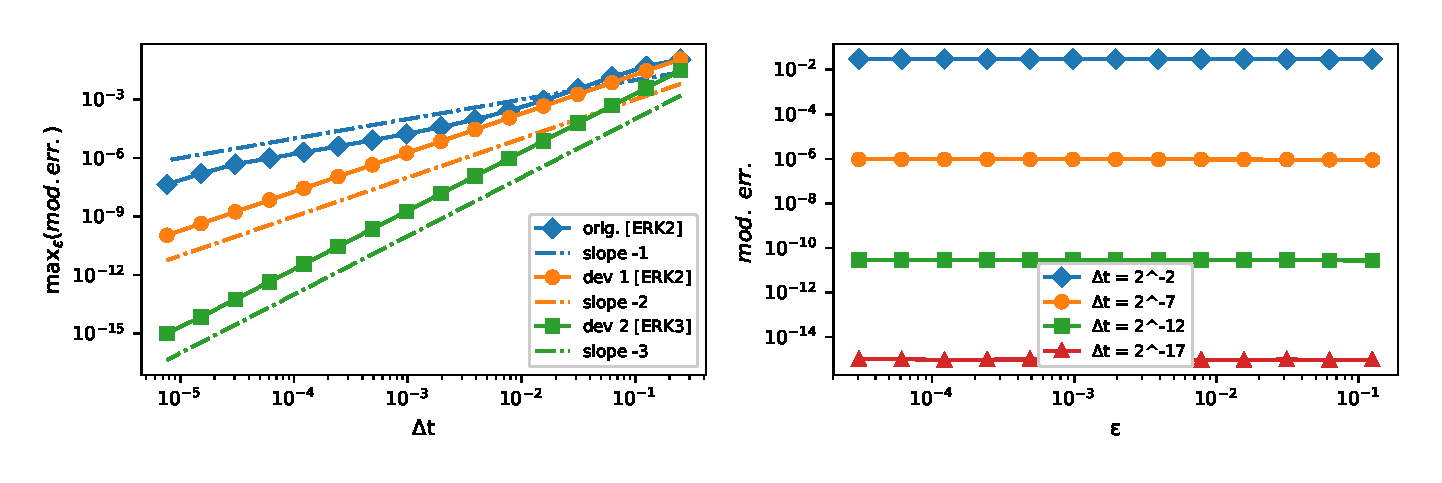
\includegraphics[width=\textwidth]{./miMa_Dissipatif/cv_oscill_max_err_and_dev2.eps}
\vspace*{-24pt}
\caption{Oscillating case: On the left, maximum error on~$\eps$ (for $\eps
= 2^{-k}$ with $k$ spanning $\{3, \ldots, 15\}$) as a function of $\Dt$
when using exponential RK schemes (abbr. ERK) of different orders. On the
right, the error as a function of $\eps$ when solving the micro-macro
problem of order~2 using ERK3.}
\label{tests_fig:oscill}
\end{figure}


\medskip
\noindent\textit{A PDE-inspired problem}\\
%
Consider a problem similar to a relaxed conservation law (as in the next
subsection) but without transport, written
\begin{equation*}
  \left\lbrace\begin{array}{ll} 
    \dot u = \tilde{u} , 
    & u(0) \in \R^{d} , \displaystyle \vphantom{\int} 
    \\ \displaystyle
    \dot{\tilde{u}} = \frac{1}{\e} \big( g(u) - \tilde{u} \big) ,
    & \tilde{u}(0) \in \R^{d} 
  \end{array}\right.
\end{equation*}
for some smooth map $g: \R^{d} \mapsto \R^{d}$. This can be
transformed in a system of the form~\eqref{intro-eq:xz_pb} by setting~$x =
u$ and $z = g(u) - \tilde{u}$, yielding the problem 
\begin{equation} \label{sec:tests:eq:hyperb_ode}
  \left\lbrace\begin{array}{ll} \displaystyle \vphantom{\int}
    \dot x = g(x) - z , 
    & x(0) = u(0) , \\ \displaystyle
    \dot z = -\frac{1}{\e} z + g'(x) \big( g(x) - z \big) ,
    & z(0) = g(u(0)) - \tilde{u}(0) .
  \end{array}\right.
\end{equation}
The change of variable and vector field can be computed by hand up
to order~1,
\begin{equation*}
  \Omega\rk{1}_{\tau}(x,z) = \begin{pmatrix}
    x + \e e^{-\tau} z \\
    e^{-\tau} z + \e g'(x) g(x)
  \end{pmatrix} ,
\end{equation*}
\begin{equation*}
  F\rk{1}(x,z) = \begin{pmatrix}
    g(x) - \e g'(x) g(x) 
    \\
    - g'(x) z + \e \big(g'(x)^2 + g''(x)g(x) 
    - \e g''(x)g'(x)g(x) \big) z
  \end{pmatrix} .
\end{equation*}
Going to a higher order requires specific computations, as the expression
of $\frac{1}{\e} (\dpt +  A) \Omega\rk 2 _\tau(x,z)$ is verbose and
involves for instance $g(x + \e e^{-\tau}z) - g(x)$. 
It can be checked by hand that this expression involves no~$e^{-\tau
 A}$-term with the above expressions of $\Omega\rk 1$ and $F\rk 1$.
For numerical testing, we chose~$g(x) = -x^3/3$, $u(0) = 1$ and
$\tilde{u}(0) = 0$. The micro-macro problem was computed up to order~2. 

\begin{figure}
  \vspace*{-12pt}
  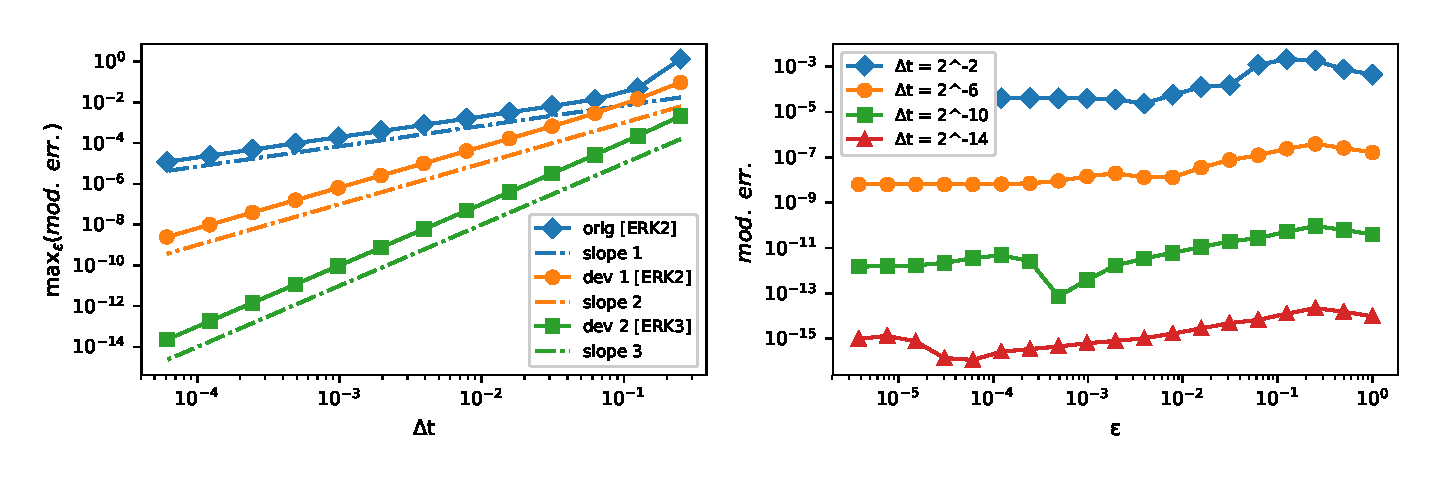
\includegraphics[width=\textwidth]{./miMa_Dissipatif/hyperb_ode.eps}
  \vspace*{-24pt}
  \caption{PDE-inspired problem: On the left, maximum error on~$\eps$ (for
  $\eps = 2^{-k}$ with $k$ spanning $\{1, \ldots, 18\}$) as a function of
  $\Dt$ when using exponential RK schemes (abbr. ERK) of different orders.
  On the right, the error as a function of $\eps$ when solving the
  micro-macro problem of order~2 using ERK3.}
  \label{tests_fig:hyperb_ode}
\end{figure}

\medskip
\noindent\textit{Results}\\
%
Figures~\ref{tests_fig:oscill} and~\ref{tests_fig:hyperb_ode} showcase the
phenomenon of order reduction when solving the original
problem~\eqref{test-pb:xz_oscil}: Despite using a scheme of order 2, the
error depends of $\eps$ in such a way that there exists no constant $C$
such that the error is bounded by $C\Dt^2$ for all $\eps$. However there
exists $C$ such that the error is bounded by $C\Dt$. In that case, we
cannot say that the error is of \textit{uniform} order~2, as this would
require the error to be independent of $\eps$.

This order reduction disappears when solving the micro-macro problem, as
can be seen on the right-hand side of the figures for a decomposition of
order 2. Furthermore, the theoretical orders of convergence from
Theorem~\ref{sec:mima:subsec:ua:thm:ua} are confirmed. Indeed, using a
scheme of order 2 (resp. 3) on the micro-macro problem of order 1 (resp.
2) generates a uniform error of the expected order of convergence, with no
order reduction. 



\subsection{Discretized hyperbolic partial differential equations}
\label{sec:tests:subsec:pde}
\hspace*{1em}

\renewcommand{\xvar}{\rho}
\renewcommand{\zvar}{z}
\noindent\textit{The telegraph equation}\\
%
\begin{figure}
\centering
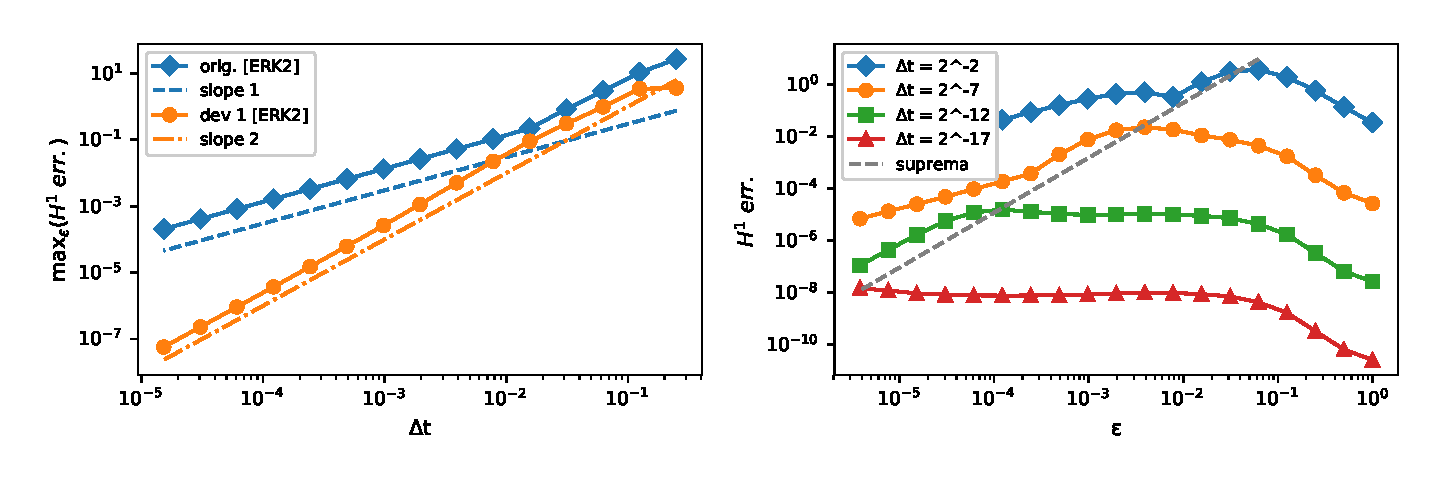
\includegraphics[width=\textwidth]{./miMa_Dissipatif/cv_telegraph_erk2.eps}
\vspace*{-24pt}
\caption{Telegraph equation: Absolute $H^1$ error on the solution of~\eqref{test_eq:cont_telegraph} computed by an ERK3 scheme. Supremum on $\eps$ as a function of $\Dt$ (left) and evolution of this error as a function of $\eps$ for the 1st-order decomposition (right). }
\label{test_fig:telegraph}
\end{figure}%
%
Using a spectral decomposition, we solve the problem, for $(t,x) \in [0,T] \times \R/2\pi\mathbb{Z}$, 
\begin{equation*} 
\left\{ \begin{array}{l}
\dpt \xvar + \dpx j = 0 , \\ \displaystyle
\dpt j + \frac{1}{\eps} \dpx \xvar = -\frac{1}{\eps} j , 
\end{array} \right. 
\end{equation*}
by setting $z = j + (1 - \alpha \eps \Delta)^{-1} \dpx z$, yielding 
problem~\eqref{pde_pb:telegraph}. The micro-macro decomposition of 
order~$1$ is summarized in Property~\ref{pde_prop:telegraph}, and its 
construction is detailed in Subsection~\ref{pde_subsec:telegraph}. 
%
Implementations are conducted using $\alpha = 2$, space frequencies are 
bounded by $k_{\max} := 12$, and initial data is $\xvar(0,x) = 
e^{\cos(x)}, \ j(0,x) = \frac{1}{2} \cos^3 (x)$. 

Results can be seen in Figure~\ref{test_fig:telegraph} when using a scheme
of order 2. When solving the original problem, the uniform order
degenerates from~2 to~1. When considering the micro-macro problem, the
order of convergence is not reduced and stays of order~2. Although it
varies with $\eps$ when considering a fixed $\Dt$, when considering the
supremum on~$\e$, there is no order reduction. The dashed slope on the
right plot interpolates the position of the supremum of the error for each
fixed $\Dt$. While the error seems to improve for $\e \ll \Dt$, this does
not cause any order reduction. This is stronger than the property of
preservation of asymptotes (which ERK schemes have,
see~\cite{dimarco.2011.exponential}), since AP schemes only need to be
well-defined in the limit $\e \rightarrow 0$. For them, this supremum does
not need to be bounded.
%
It appears that the relationship between the error bound and the stiffness
of the linear operator is rather complex when using exponential RK schemes
(again, see~\cite{hochbruck.2005.explicit} for details). 



\renewcommand{\Dx}{\Delta x}
\renewcommand{\rlxcont}{\tilde{u}}
\renewcommand{\rlxdisc}{\tilde{U}}
\renewcommand{\xvar}{U_1}
\renewcommand{\zvar}{U_2}
\medskip
\noindent\textit{Relaxed conservation law}\\
%
\begin{figure}
\centering
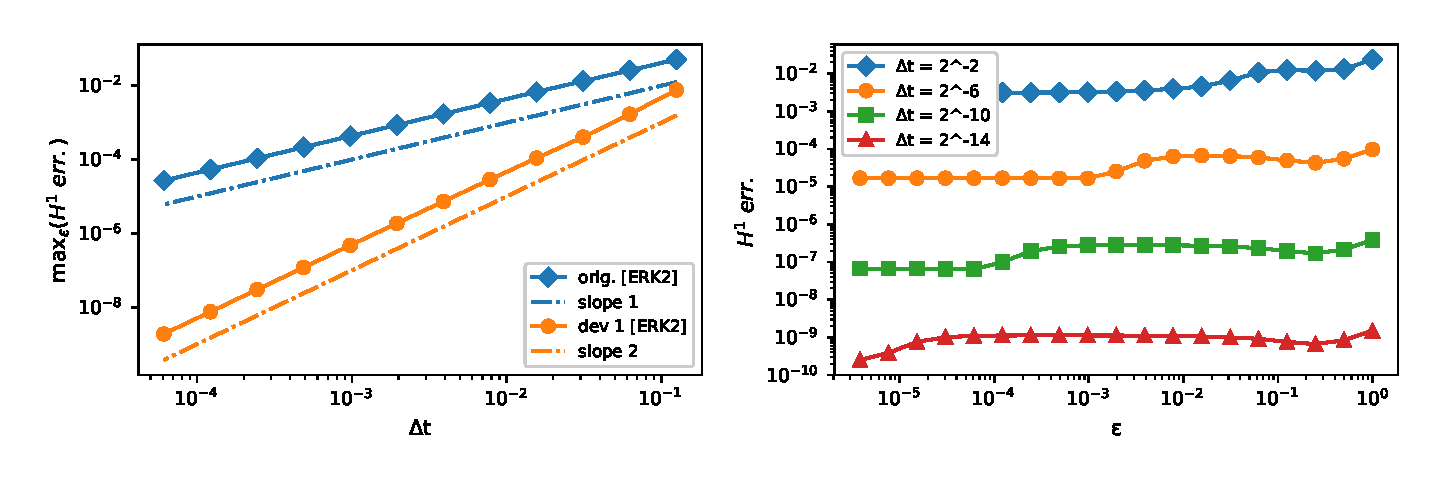
\includegraphics[width=\textwidth]{./miMa_Dissipatif/cv_hyperb_erk2.eps}
\vspace*{-24pt}
\caption{Relaxed Burgers-type problem: Maximum modified $H^1$ error (for $\eps$ spanning $1$ to $2^{-18}$ using an ERK3 scheme as a function of $\Dt$ (left), and $H^1$ error as a function of $\eps$ for the micro-macro problem of order~1 (right).}
\label{test_fig:sqr_results}
\end{figure}%
%
Our second test case is a hyperbolic problem for $(t,x) \in [0,T] \times \R/2\pi \mathbb Z$, 
\begin{equation*} %\label{test_eq:cont_hyperb_uv}
\left\{ \begin{array}{l}
\dpt u + \dpx \rlxcont = 0 , \\ \displaystyle
\dpt \rlxcont + \dpx u = \frac{1}{\eps}(g(u) - \rlxcont) ,
\end{array} \right .
\end{equation*}
discretized with finite volumes and written in the form of~\eqref{intro-eq:xz_pb} 
by setting $u_1 = u$ and $u_2 = \tilde{u} - g(u)$ 
the $x\eeps$- and the $z\eeps$-component respectively. 
The micro-macro expansion is computed to order~$1$ using the strategy detailed in Subsection~\ref{pde_subsec:conservation}. 

For our tests, following~\cite{hu.2021.uniform}, we consider 
$ g(u) = bu^2 $ 
with $b = 0.2$. 
Simulations run to a final time $T = 0.25$ and the mesh size is fixed: $N = 16$. 
Initial data is $u(0,x) = \frac{1}{2} e^{\sin(x)}$ and $\rlxcont(0,x) = \cos(x)$. 
The reference solution was computed up to a precision $10^{-12}$ using an ERK2 scheme. 
Convergence results are presented in Figure~\ref{test_fig:sqr_results}, 
confirming theoretical results once more. 

It should be said again that our approach does not study the error in space, only in time. 
For instance, the relationship between the error bound and the grid size is not considered. 
Further studies will be conducted, especially considering CFL conditions, $L^2$ and $H^1$ norms, and computational costs. 


\subsection{Perspectives} 
\label{sec:tests:subsec:thoughts}

\hspace*{1em}

\noindent\textit{Computing cost}\\
%
Note that when using a given scheme, solving a single step is much more
costly for the micro-macro problem than for the direct problem: Not only
is the system size doubled, but the functions implicated require more
computing power to obtain a single value (especially the defect,
see~\eqref{sec:pde:subsec:csv:eq:eta1} for instance). It is therefore 
plausible to think that our method is best for computing values during the
transient phase, after which it is possible to solve the original problem 
with uniform accuracy. 

The regularized derivation $\big( I_N - 2\eps D^2 \big)^{-1} D$ which
appears in the micro-macro problem of the relaxed hyperbolic system may be
prohibitively costly to compute for some schemes such as WENO, for which
the derivation operator is non-linear. However we may be able to work
around this, as the goal of the relaxation term is only to dampen
high-frequencies, and as such inverting any discrete Laplace operator
should suffice, independently of the scheme used to discretize the
transport. Clearly, the subject of utilizing such regularizations for
numerical purposes is complex and beyond the scope of this paper.


\medskip
\noindent\textit{Near-equilibrium convergence}\\
%
\begin{figure}
\centering
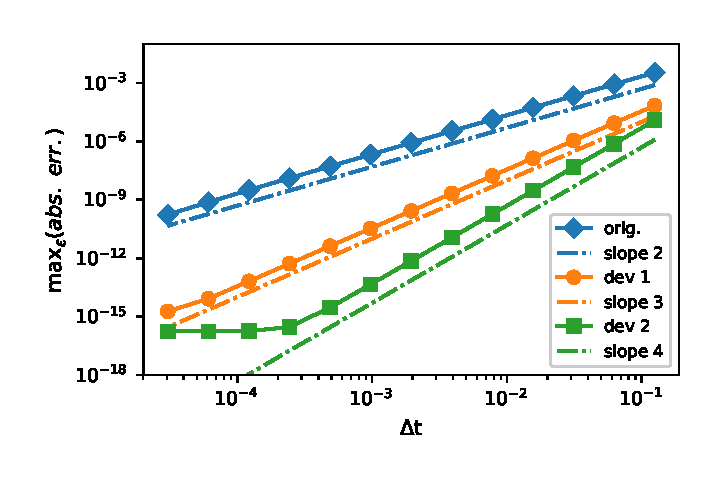
\includegraphics[width=0.48\textwidth]{./miMa_Dissipatif/ord_gain_oscill.eps}
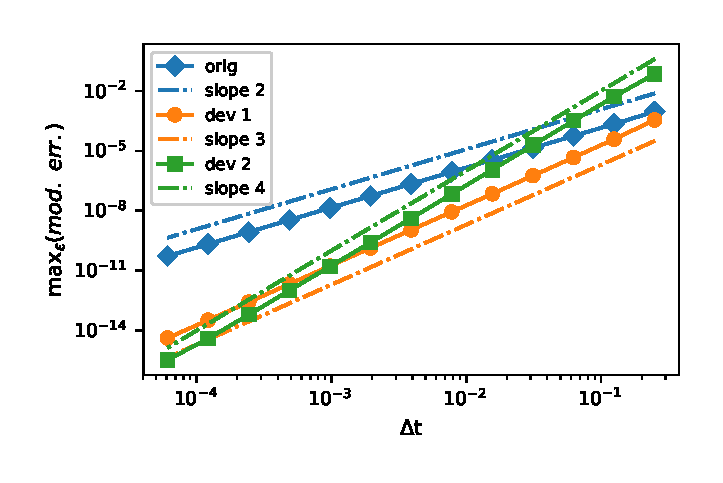
\includegraphics[width=0.48\textwidth]{./miMa_Dissipatif/ord_gain_hyperb_ode.eps}
\\
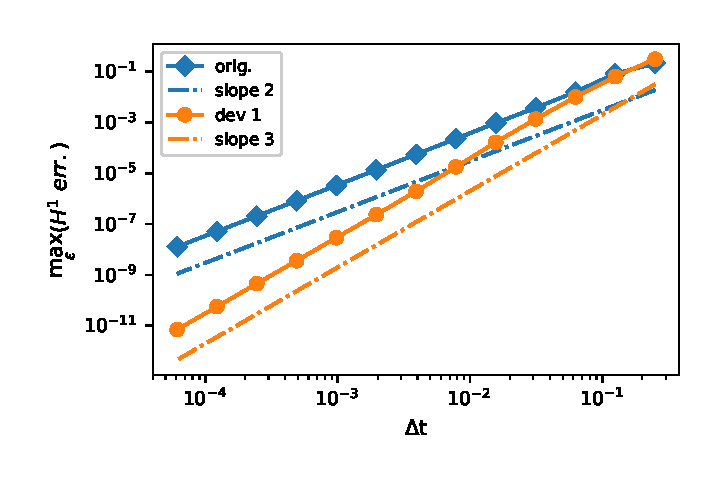
\includegraphics[width=0.48\textwidth]{./miMa_Dissipatif/ord_gain_telegraph.eps}
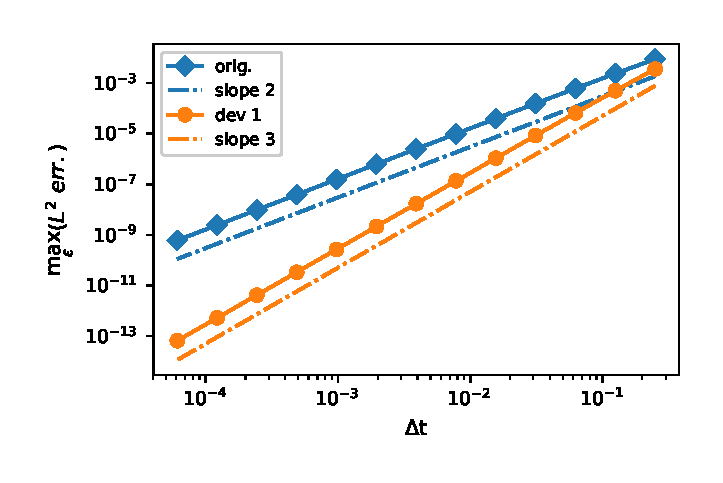
\includegraphics[width=0.48\textwidth]{./miMa_Dissipatif/ord_gain_cons_law.eps}
\vspace*{-10pt}
\caption{In reading order, errors when solving the oscillating toy
problem, the PDE-inspired problem, the telegraph equation and the relaxed
conservation law. All systems start near equilibrium and are solved with
exponential Runge-Kutta schemes of the observed order of convergence.}
\label{test_fig:order_gain}
\end{figure}%
%
If one chooses an initial condition $z\eeps(0) = 0$ in~\eqref{intro-eq:xz_pb}, 
then it is close to the center manifold up to $\bigO(\eps)$, 
and Problem~\eqref{intro-pb:full_pb_on_u} can be solved with uniform accuracy of order 2 
but only when considering the absolute error $|\cdot|$, 
not the modified error $\modnorm{\,\cdot\,}$ from~\eqref{mima_def:modnorm}. 
The same behaviour is observed for the telegraph equation when setting $j(0,x) = -\dpx \rho(0,x) $, meaning $z = \bigO(\eps)$. 
This would theoretically mean that we need to push the micro-macro 
decompositions up to order 2 if we want to improve the order of 
convergence. However, this is not the case: uniform accuracy of order 3 is 
obtained from an expansion of order 1 for all test cases. 
%
This ``order gain'' also propagates to our micro-macro decomposition of order~2 
for the oscillating toy problem. 
These results can be seen in Figure~\ref{test_fig:order_gain} 
and will be studied in future works. 
